\documentclass[a4paper,14pt]{extarticle}

\usepackage{geometry}
\usepackage[T2A]{fontenc}
\usepackage[utf8]{inputenc}
\usepackage[english,russian]{babel}
\usepackage{amsmath}
\usepackage{amsthm}
\usepackage{amssymb}
\usepackage{mathtools}
\usepackage{fancyhdr}
\usepackage{setspace}
\usepackage{graphicx}
\usepackage{colortbl}
\usepackage{xcolor}
\usepackage{tikz}
\usepackage{pgf}
\usetikzlibrary{arrows.meta,positioning,fit,shapes.geometric,calc}
\usepackage{subcaption}
\usepackage{caption}
\usepackage{float}
\usepackage{listings}
\usepackage{indentfirst}
\usepackage{enumitem}
\usepackage{booktabs}
\usepackage{array}
\usepackage{longtable}
\usepackage{pdflscape}
\usepackage{multirow}
\usepackage[flushleft]{threeparttable}

\usepackage[
backend=biber,
style=numeric,
sorting=none,
maxbibnames=99
]{biblatex}
\addbibresource{refs.bib}
\ExecuteBibliographyOptions{url=true,urldate=comp,doi=false,isbn=false}
\usepackage[colorlinks,citecolor=blue,linkcolor=blue,bookmarks=false,hypertexnames=true,urlcolor=blue]{hyperref}

\numberwithin{table}{section}
\numberwithin{figure}{section}
\numberwithin{equation}{section}

\graphicspath{{graphics/}{../outputs/}{../outputs/chain_grouping_llm_model_experiments/figures/}{../outputs/survey_audio_feedback/figures/}}

\geometry{left=2.5cm}
\geometry{right=1.0cm}
\geometry{top=2.0cm}
\geometry{bottom=2.0cm}
\setlength{\parindent}{1.25cm}
\renewcommand{\baselinestretch}{1.5}

\newcommand{\bibref}[3]{\hyperlink{#1}{#2 (#3)}}
\addto\captionsrussian{\def\refname{Список литературы}}
\addto\captionsrussian{\renewcommand{\contentsname}{Содержание}}

\captionsetup[figure]{name={Рисунок},labelsep=endash,justification=centering}
\captionsetup[table]{name={Таблица},labelsep=endash,justification=raggedright,singlelinecheck=false}

\renewcommand{\theenumi}{\arabic{enumi}}
\renewcommand{\labelenumi}{\arabic{enumi})}
\renewcommand{\theenumii}{.\arabic{enumii}}
\renewcommand{\labelenumii}{\arabic{enumi}.\arabic{enumii}.}
\renewcommand{\theenumiii}{.\arabic{enumiii}}
\renewcommand{\labelenumiii}{\arabic{enumi}.\arabic{enumii}.\arabic{enumiii}.}
\setlist[enumerate,1]{label=\arabic*),leftmargin=1.25cm,labelsep=0.35em,itemsep=0pt,topsep=0.3\baselineskip,parsep=0pt,partopsep=0pt}
\setlist[itemize]{leftmargin=1.25cm,itemsep=0.15\baselineskip,topsep=0.2\baselineskip}

\lstset{basicstyle=\ttfamily\small,breaklines=true,frame=single,columns=fullflexible}

\definecolor{hseblue}{HTML}{005BBB}
\definecolor{hselight}{HTML}{D7ECFF}
\definecolor{hsemid}{HTML}{5AA9E6}
\definecolor{hsedark}{HTML}{0F2F4F}
\definecolor{softgray}{HTML}{F5F8FC}

\newcommand{\todo}[1]{\textcolor{red}{[TODO: #1]}}

\begin{document}

\begin{titlepage}
\newpage

{\setstretch{1.0}
\begin{center}
ПРАВИТЕЛЬСТВО РОССИЙСКОЙ ФЕДЕРАЦИИ\\
ФГАОУ ВО НАЦИОНАЛЬНЫЙ ИССЛЕДОВАТЕЛЬСКИЙ УНИВЕРСИТЕТ\\
«ВЫСШАЯ ШКОЛА ЭКОНОМИКИ»
\\
\bigskip
Факультет компьютерных наук\\
Образовательная программа «Искусственный интеллект»
\end{center}
}

\vspace{7em}

\begin{center}
{\bf ВЫПУСКНАЯ КВАЛИФИКАЦИОННАЯ РАБОТА}\\
{\bf Программный проект на тему:}\\
{\bf Разработка системы генерации тифлокомментариев на основе данных футбольных матчей}\\
\end{center}

\vspace{2em}

{\bf Выполнил студент: \vspace{2mm}}

{\setstretch{1.1}
\begin{tabular}{l@{\hskip 1.5cm}l}
группы \#МИИ243, 2 курса & Мясникова Ангелина Андреевна
\end{tabular}}

\vspace{1em}
{\bf Принял руководитель ВКР: \vspace{2mm}}

{\setstretch{1.1}
\begin{tabular}{@{}p{0.82\textwidth}@{}}
Дурыгин Олег Дмитриевич\\
Руководитель направления по исследованию данных\\
ПАО «Сбербанк»
\end{tabular}}


\vspace{\fill}

\begin{center}
Москва 2026
\end{center}

\end{titlepage}

\newpage
\setcounter{page}{2}

\tableofcontents
\newpage

% =========================
% АННОТАЦИЯ
% =========================
\section*{Аннотация}
\addcontentsline{toc}{section}{Аннотация}

Работа посвящена разработке прототипа системы автоматической генерации русскоязычных тифлокомментариев к футбольному матчу на основе структурированных событийных данных StatsBomb. В отличие от видеоориентированных подходов, рассматриваемый прототип строит комментарий без доступа к видеоряду: входом служат JSON-события матча, включающие тип действия, временную метку, координаты, участников эпизода, исход действия и при наличии данные StatsBomb~360. Основное внимание уделяется не только генерации текста языковой моделью, но и подготовке входного представления: стандартизации координат с учётом смены сторон, фильтрации некорректных 360-кадров, построению компактных цепочек событий и отбору эпизодов, пригодных для озвучивания.

В работе предложен пайплайн, включающий предобработку данных, формирование нескольких стратегий группировки событий, эвристическую soft-разметку важности эпизодов, обучение моделей отбора на 51 матче Евро-2024, генерацию комментариев через LLM и последующую сборку аудиодорожки с помощью Silero TTS. Экспериментальная часть сравнивает стратегии формирования эпизодов и модели отбора, а также оценивает форматную корректность и фактическую пригодность LLM-комментариев. Практический результат работы --- воспроизводимый прототип, позволяющий получить структурированные JSON-комментарии и аудиодорожку для выбранных матчей.

\section*{Ключевые слова}
\addcontentsline{toc}{section}{Ключевые слова}

Тифлокомментирование; аудиоописание; футбольные события; StatsBomb; StatsBomb 360; data-to-text generation; спортивная суммаризация; языковые модели; soft labels; CatBoost; Silero TTS.

\newpage

% =========================
% ВВЕДЕНИЕ
% =========================
\section{Введение}

Тифлокомментарий --- это специальный формат аудиоописания, предназначенный для людей с нарушениями зрения. В спортивной трансляции он решает практическую задачу: передать слушателю, где находится мяч, кто выполняет действие и чем завершается эпизод. В отличие от обычного спортивного репортажа, такой комментарий не столько оценивает игру, сколько помогает слушателю представить происходящее на поле. Поэтому он должен быть кратким, нейтральным и опираться только на проверяемые факты: где мяч, кто действует и как меняется эпизод.

Актуальность задачи связана с тем, что доступность спортивных трансляций постепенно становится частью международной и российской практики. На международном уровне FIFA обеспечивала аудиодескриптивное комментирование для слепых и слабовидящих болельщиков во время Клубного чемпионата мира FIFA 2025~\cite{fifaClubWorldCupADC2025}. В европейском футболе развитие таких сервисов поддерживается CAFE (Centre for Access to Football in Europe): организация совместно с футбольными структурами продвигает обучение аудиодескриптивных комментаторов и внедрение сервиса для слепых и слабовидящих болельщиков~\cite{uefaCafeADC2018}. В России также появляются инфраструктурные решения: приложение «Особый взгляд» предоставляет доступ к адаптированным аудиодорожкам и прямому тифлокомментированию, включая спортивные матчи~\cite{specialViewAppPatent2025,specialViewFootballRussia2024}; в российских футбольных материалах отмечается сотрудничество «Спартака», «Локомотива» и «Крыльев Советов» с этим приложением~\cite{sportsruTiflo2024}. Кроме того, Okko развивает тифлокомментирование в спортивных трансляциях: сервис сообщает о запуске тифлокомментариев для ключевых матчей Лиги чемпионов и о дальнейшем расширении таких дорожек~\cite{okkoTiflo2025}. Всё это показывает, что задача автоматизации и масштабирования тифлокомментариев имеет не только исследовательскую, но и практическую социальную значимость.

\begin{figure}[H]
\centering

\includegraphics[width=0.82\textwidth]{fan_audio_description.png}
\caption{Использование устройства для прослушивания тифлокомментария во время спортивного мероприятия}
\label{fig:fan-audio-description}
\end{figure}

Футбольный матч представляет собой сложный поток событий. Один матч содержит тысячи записей: передачи, приёмы мяча, ведение, давление, фолы, удары, стандарты, действия вратаря. Большая часть этих событий не требует отдельной реплики: если описывать каждое действие, комментарий станет перегруженным и непригодным для восприятия. Поэтому задача автоматического тифлокомментирования не сводится только к генерации текста. Перед генерацией необходимо решить задачу отбора: какие эпизоды стоит озвучивать, как объединять отдельные события в смысловые цепочки и какой контекст передавать языковой модели.

В данной работе рассматривается event-based постановка: система получает не видео, а структурированный журнал событий StatsBomb. Такой подход имеет несколько преимуществ. Во-первых, он дешевле и воспроизводимее мультимодального анализа видео. Во-вторых, многие факты уже представлены в структурированном виде: тип действия, координаты, игрок, исход передачи или удара. В-третьих, такой формат позволяет явно контролировать фактическую опору комментария и снижать риск галлюцинаций языковой модели.

Однако у событийных данных есть и ограничения. Координаты StatsBomb задаются в фиксированной системе поля, но команды меняют стороны во втором тайме. Значит, понятия «вперёд», «назад», «своя половина», «чужая штрафная» должны вычисляться относительно команды и периода. Кроме того, данные StatsBomb~360 иногда оказываются геометрически несогласованными с событием, поэтому требуется отдельная фильтрация таких кадров. Наконец, связанные события могут образовывать слишком длинные цепочки, которые неудобно передавать в LLM: модель начинает пересказывать поток действий вместо короткого комментария.

Цель работы --- разработать и экспериментально исследовать прототип системы генерации русскоязычных тифлокомментариев к футбольным матчам по данным StatsBomb JSON.

Для достижения цели решаются следующие задачи:

\begin{enumerate}
    \item изучить литературу по автоматическому аудиоописанию, генерации спортивных комментариев и data-to-text generation;
    \item разработать процедуру стандартизации событий и координат с учётом смены сторон в таймах;
    \item реализовать фильтрацию некорректных StatsBomb~360 кадров и визуальную проверку стандартизации;
    \item предложить стратегии группировки событий в эпизоды и сравнить их по длине, стоимости и пригодности для LLM;
    \item построить эвристическую soft-разметку важности эпизодов и обучить модели отбора;
    \item сформировать LLM-payloads и системный промпт для генерации тифлокомментария;
    \item оценить качество LLM-ответов и собрать аудиодорожку с помощью Silero TTS;
    \item подготовить прототип визуального интерфейса для просмотра событий и результатов.
\end{enumerate}

Новизна работы состоит в адаптации пайплайна генерации аудиоописаний к русскоязычному футбольному тифлокомментарию по event JSON без видеоряда, а также в экспериментальном сравнении нескольких стратегий формирования эпизодов и отбора комментариев на всех 51 матчах Евро-2024.

Дальнейшая структура работы следующая. В Разделе~\ref{sec:literature} приведён обзор литературы. В Разделе~\ref{sec:data} описаны данные и стандартизация. В Разделе~\ref{sec:methodology} формализуется пайплайн формирования эпизодов и отбора. В Разделе~\ref{sec:experiments} приводятся эксперименты. В Разделе~\ref{sec:system} описан программный прототип. В заключении сформулированы результаты и направления дальнейшей работы.

% =========================
% ОБЗОР ЛИТЕРАТУРЫ
% =========================
\section{Обзор литературы}\label{sec:literature}

Обзор построен от наиболее близких к задаче работ к более общим. Сначала рассматриваются исследования, где комментарий строится по структурированным событиям или текстовым трансляциям без видео. Затем обсуждаются работы по спортивной суммаризации, отбору значимых событий и data-to-text generation. Далее переходим к конкретным датасетам, вопросам временного выравнивания и мультимодальным расширениям. В конце выделяются ограничения существующих подходов и обосновывается вклад настоящей работы.

\subsection{Генерация комментариев по структурированным событиям}

Одной из наиболее близких к поставленной задаче работ является~\cite{wang2022commentary}, где авторы рассматривают генерацию комментариев по журналам событий киберспортивных матчей в League of Legends. Вход~--- структурированные игровые события с атрибутами; выход~--- текстовые комментарии в духе живого репортажа. Работа примечательна тем, что видео здесь вообще отсутствует: всё, что доступно системе,~--- это последовательность записей о действиях игроков. Авторы показывают, что такого входа достаточно для осмысленной генерации, если правильно выбирать ключевые события и поддерживать связность повествования.

Эта постановка очень близка к задаче настоящей работы. StatsBomb JSON по своей структуре устроен аналогично: каждая запись описывает одно действие на поле, содержит тип события, время, пространственные координаты и дополнительные поля. Разница лишь в домене~--- футбол против киберспорта,~--- но методологически оба сценария относятся к одному классу задач. Ключевой вывод из~\cite{wang2022commentary}: структурированные события достаточно выразительны для комментария при условии, что вход нормализован и содержательно отфильтрован.

Несколько иной угол зрения предлагает работа~\cite{racing}, где исследуется генерация комментариев для гоночных игр на основе комбинации числовых параметров, текстовых описаний и визуальных признаков. Интересно, что авторы отдельно исследуют вклад каждой модальности и приходят к выводу: структурированные числовые данные и текст дают значительную часть полезного сигнала, тогда как визуальный канал улучшает результат, но не является незаменимым. Для настоящей работы это важно как косвенное подтверждение того, что event-based подход жизнеспособен сам по себе.

\subsection{Спортивные новости и live text commentary}

Другое направление, непосредственно связанное с задачей,~--- это построение спортивных новостей и коротких отчётов по текстовым лентам трансляции. В работе~\cite{zhang2016sportsnews} авторы предлагают метод автоматического формирования матчевой новости из live text commentary: системы, которые в реальном времени выдают короткие текстовые сообщения о происходящем на поле. Задача сформулирована как extractive summarization: из потока сообщений нужно отобрать наиболее информативные и собрать из них связный отчёт.

Ключевое наблюдение этой работы состоит в том, что простое объединение сообщений не работает: большинство из них либо дублируют информацию, либо содержат незначительные детали. Авторы предлагают использовать признаки, связанные с изменением счёта, временем матча и типом события, чтобы оценивать значимость фрагментов. Для настоящей работы это важно по двум причинам: во-первых, подход строится исключительно на текстовых данных; во-вторых, он явно разделяет задачи отбора и генерации, что соответствует архитектуре, выбранной в данной работе.

Продолжением этой линии является~\cite{contentselection}, где проблема content selection для спортивных новостей рассмотрена подробнее. Авторы анализируют, какие типы событий чаще попадают в итоговые отчёты и почему, выделяют признаки значимости и показывают, что хороший отбор контента влияет на итоговое качество текста сильнее, чем улучшение модели генерации. Этот вывод хорошо согласуется с практическим опытом работы над настоящим проектом: изменение правил фильтрации событий даёт более заметный эффект, чем перебор различных промптов.

\subsection{Спортивная суммаризация}

В работе~\cite{sportssum2} задача построения спортивных новостей по live text commentary рассматривается с другой стороны. Авторы критически анализируют качество существующих датасетов и показывают, что многие из них содержат шумную псевдоразметку, полученную автоматически. Это делает прямое обучение на таких данных проблематичным: модель учится воспроизводить артефакты разметки, а не реальные закономерности журналистского текста. В результате предлагаются методы очистки датасета и контроля качества пар «лента~--- новость».

Для настоящей работы это наблюдение особенно ценно. В задаче тифлокомментирования размеченных пар «события~--- комментарий» практически не существует, тем более для русскоязычного контекста. Значит, рассчитывать на обучение с учителем на готовых парах не приходится. Это подталкивает к подходу, основанному на чётких правилах отбора событий и generation через языковую модель с тщательно подготовленным промптом.

Важным ресурсом в этом контексте является работа о Chinese sports summarization~\cite{chinesesports}, где схожая задача решается для китайского языка. Авторы показывают, что текстовые данные трансляций, даже без видео, позволяют строить суммаризацию достаточного качества при условии хорошей нормализации входа. Кроме того, в работе обсуждаются проблемы, специфичные для нелатинских языков,~--- например, токенизация и морфологическая неоднозначность. Эти наблюдения актуальны и для русскоязычного тифлокомментирования.

\subsection{Отбор значимых событий}

В задаче тифлокомментирования отбор событий~--- не вспомогательный этап, а центральный. Большую часть матча составляют рутинные эпизоды: короткие пасы в центре поля, позиционное перемещение без мяча, неактивные фазы. Если комментировать всё подряд, слушатель окажется в информационном шуме. Если быть слишком избирательным~--- пропустит важные моменты.

Исследования по выделению значимых событий в спортивных данных~\cite{contentselection,zhang2016sportsnews} формулируют ряд устойчивых критериев: изменение счёта, нахождение мяча в штрафной зоне, удары по воротам, стандартные положения, смена владения в опасной зоне. В работе рассматривается смежная задача~--- автоматическое распознавание событий из текста комментария,~--- и авторы показывают, какие типы действий чаще всего упоминаются в репортажах. Этот обратный анализ даёт полезные подсказки о том, что считается «комментируемым» в реальной практике.

Отдельную роль играет временн\'{а}я близость событий. Передача, приём и удар~--- это не три независимых события, а единый эпизод атаки, и комментировать их стоит вместе. В работе~\cite{lfc2025} авторы специально выстраивают датасет с учётом группировки событий в эпизоды и показывают, что модели, обученные на эпизодах, генерируют более связный текст, чем модели, работающие с отдельными событиями. Именно поэтому в настоящей работе сделан акцент на построении окон контекста, а не на пообъектной обработке.

\subsection{Генерация текста по данным}

Задача data-to-text generation изучается в NLP достаточно давно и имеет хорошо разработанную методологию. Ранние работы~\cite{data2text} строили детерминированные шаблонные системы: каждому типу записи соответствовал набор заготовленных фраз с подстановкой значений. Такой подход прост в реализации и даёт предсказуемый результат, но плохо обобщается на разнообразные ситуации.

Позже появились нейросетевые подходы~\cite{record2text}, где модель обучается преобразовывать таблицы или JSON-структуры в текст. Современные языковые модели делают этот переход ещё более плавным: при правильно составленном промпте они способны интерпретировать структурированные данные и генерировать по ним связные фразы без явного обучения на парах «вход~--- выход». Именно этот сценарий используется в данной работе, где языковая модель получает на вход заранее подготовленное окно событий и выдаёт короткий комментарий.

Принципиальное наблюдение из литературы по data-to-text~\cite{data2text,record2text}: качество выходного текста в значительной мере определяется качеством входного представления. Если данные поданы с лишними полями, противоречивыми значениями или неверной ориентацией пространственных координат, модель либо игнорирует эти детали, либо воспроизводит ошибки. Для задачи тифлокомментирования это означает, что предобработка и стандартизация~--- не технический ритуал, а содержательная часть решения.

\subsection{Датасеты футбольных комментариев}

Если посмотреть, что именно сейчас доступно в качестве обучающих ресурсов для футбольного комментария, картина получается неоднородной. Датасет SoccerNet-Echoes~\cite{soccernet_echoes} представляет собой большую коллекцию аудиокомментариев, выровненных с временными метками матчей. Он предназначен прежде всего для задач speech recognition и аудиогенерации, но косвенно полезен и для тифлокомментирования: данные показывают, какие типы эпизодов чаще всего удостаиваются развёрнутого устного описания.

Датасет LFC~\cite{lfc2025} устроен иначе: в нём текстовые комментарии выровнены с координатами игроков из tracking data, что позволяет обучать и оценивать модели генерации на уровне отдельных эпизодов. Авторы специально сравнивают text-based и image-based представления футбольных событий и показывают, что текстовое кодирование позиций не уступает визуальному по итоговому качеству комментария. Это~--- прямое подтверждение того, что задача генерации тифлокомментария по событийным данным методологически состоятельна.

Открытые данные StatsBomb~\cite{statsbomb,statsbombschema} не являются датасетом комментариев в строгом смысле, но служат основным источником событийной информации в настоящей работе. Особенность формата~--- высокая детализация: по сравнению с другими открытыми источниками StatsBomb содержит данные о давлении, типах приёмов мяча, выборе зон на поле. Это делает его одним из наиболее информативных открытых форматов для футбольного анализа и удобным источником для построения тифлокомментариев.

\subsection{Автоматический футбольный комментарий}

Работа~\cite{matchtime2024} рассматривает задачу автоматической генерации комментариев к футбольным матчам и делает особый акцент на проблеме temporal alignment~--- то есть правильного соответствия между событием и моментом его описания. Авторы показывают, что даже небольшое рассогласование по времени заметно ухудшает воспринимаемое качество комментария. Кроме того, в работе сравниваются разные способы представления входных данных: текстовое описание событий, изображения поля и трекинг игроков.

Важный практический вывод~\cite{matchtime2024}: при использовании только текстовых и координатных данных модель показывает результаты, сопоставимые с мультимодальными вариантами. Это ещё раз подтверждает, что видеопоток не является обязательным компонентом системы. При этом авторы особо отмечают необходимость стандартизации координат с учётом смены сторон~--- именно та проблема, которая оказывается нетривиальной в работе с данными StatsBomb.

Другая недавняя работа по Soccer Commentary Generation~\cite{matchvoice2025} исследует генерацию комментариев для highlight clips~--- коротких видеофрагментов ключевых моментов. Здесь на первый план выходит задача alignment'а: как связать момент ролика с правильным комментарием. Авторы отмечают, что именно выравнивание, а не качество генератора текста, является узким местом существующих подходов. Для настоящей работы это важное наблюдение: задача определения нужного момента для комментария оказывается нетривиальной даже при наличии развитых генеративных моделей.

В работе~\cite{vision2026} предлагается подход к генерации комментариев с использованием knowledge-enhanced визуального рассуждения: система дополняет визуальное восприятие сценой фактическими знаниями о правилах игры, составе команд и статистике. Это интересный вектор развития, хотя для задачи тифлокомментирования существенно то, что и в этой работе событийные данные остаются основным источником структурной информации, а визуальный канал добавляет лишь дополнительный контекст.

Наиболее близкой к задаче аудиоописания футбольного матча является работа MCAD~\cite{mcad2025}, где рассматривается multimodal context-aware audio description generation for soccer. В отличие от классического спортивного комментария, MCAD ориентирована именно на описание сцены для пользователя, которому недостаточно одного видеоряда. Для настоящей работы эта постановка важна методологически: она подтверждает необходимость не только сгенерировать текст, но и выбрать момент, содержание и степень детализации описания. Отличие предлагаемого подхода состоит в том, что входом служит не видеопоток, а стандартизированный событийный JSON с координатами и 360-контекстом; это делает систему дешевле, воспроизводимее и применимой к открытым данным StatsBomb.

\subsection{Трекинг игроков и пространственный контекст}

Ряд работ рассматривает комментарий как задачу, в которой пространственная информация играет ключевую роль. В~\cite{tracking2025} используются данные трекинга игроков~--- точные траектории перемещения на поле~--- для генерации более точных пространственных описаний. Авторы показывают, что добавление трекинговой информации позволяет генератору корректно описывать относительное положение игроков, зоны прессинга и направления движения мяча.

Для данной работы это направление пока остаётся за рамками основного прототипа: StatsBomb предоставляет координаты отдельных событий, но не непрерывный трекинг. Тем не менее описанный подход задаёт возможное направление расширения: при наличии трекинговых данных систему можно дополнить более точными пространственными описаниями, не меняя общую архитектуру.

\subsection{Обзорные работы и индустриальный контекст}

Обзор~\cite{aigccsurvey} систематизирует задачи, датасеты и методы автоматической генерации игровых комментариев: от шахмат и го до футбола и киберспорта. Авторы выделяют несколько сквозных проблем: отсутствие унифицированных метрик оценки, сложность выравнивания комментария с событиями, ограниченное количество качественных датасетов. Обзор подтверждает, что задача генерации комментариев по событийным данным является самостоятельным направлением с устойчивым корпусом работ, а не вспомогательной задачей компьютерного зрения.

С практической стороны интерес представляет опыт индустриальных систем~\cite{industry2026}. Реальные продукты для автоматического комментирования матчей строятся на многослойных пайплайнах: ингестиция событий, фильтрация по значимости, формирование контекста, генерация текста и постпроверка. Простая подача сырых данных напрямую в языковую модель в промышленных системах не используется именно потому, что это даёт нестабильный и трудно воспроизводимый результат. Этот опыт подтверждает архитектурные решения, принятые в данной работе.

\subsection{Ограничения и вклад настоящей работы}

Анализ литературы выявляет несколько устойчивых ограничений, характерных для большинства существующих работ.

Во-первых, практически все исследования ориентированы на англоязычные данные. Русскоязычные футбольные комментарии~--- это отдельный жанр с собственной лексикой, стилистикой и языковыми нормами. Готовых размеченных данных для русского языка практически нет, а результаты, полученные на английских датасетах, нельзя переносить напрямую.

Во-вторых, многие исследования по комментированию матчей де-факто предполагают наличие видеопотока или как минимум трекинговых данных высокого разрешения. Задача, сформулированная только на основе event JSON, решается значительно реже~--- хотя, как показывает ряд работ~\cite{wang2022commentary,lfc2025,matchtime2024}, именно такая постановка вполне осмысленна и практически реализуема.

В-третьих, в большинстве работ значительный акцент делается на качестве генеративной модели, тогда как предобработка входа~--- стандартизация координат, фильтрация событий, построение окон~--- остаётся в тени или описывается кратко. Между тем именно эти этапы во многом определяют практическое качество системы.

Настоящая работа закрывает эти пробелы применительно к конкретному сценарию: русскоязычный тифлокомментарий по данным StatsBomb JSON, без видео, с акцентом на надёжную предобработку и структурированное формирование контекста.

\section{Данные и предобработка}\label{sec:data}

\subsection{Источник данных}

В экспериментах используются все 51 матча Евро-2024 из StatsBomb Open Data. Для каждого матча доступны события \texttt{events} и при наличии данные StatsBomb~360. Отдельно выделяется подмножество матчей для финальной генерации и озвучивания: матч открытия Германия --- Шотландия и матчи финальной стадии.

Единицей исходных данных является одно футбольное событие. Это JSON-запись, в которой указано, когда произошло действие, какая команда и игрок участвовали, где находился мяч на поле и какой был исход действия. Например, для передачи в данных есть начальная координата \texttt{location}, конечная координата \texttt{pass.end\_location}, получатель \texttt{pass.recipient}, высота передачи \texttt{pass.height} и, если передача неудачна, поле \texttt{pass.outcome}. Для ведения мяча аналогично используется \texttt{carry.end\_location}, для удара --- поля внутри \texttt{shot}.

Данные StatsBomb~360 задают не новое событие, а дополнительный моментный снимок расположения игроков в тот же момент времени. В нём есть \texttt{freeze\_frame}: координаты видимых игроков, признаки \texttt{teammate}, \texttt{actor}, \texttt{keeper}, а также \texttt{visible\_area} --- многоугольник видимой области камеры. У части событий 360-данных нет; у части они есть, но могут быть геометрически ошибочными, поэтому такие кадры дополнительно проверяются.

\begin{table}[H]
\caption{Основные поля исходных данных StatsBomb}
\label{tab:statsbomb-fields}
\centering
\small
\begin{tabular}{p{0.23\textwidth}p{0.28\textwidth}p{0.40\textwidth}}
\toprule
\textbf{Блок} & \textbf{Примеры полей} & \textbf{Смысл для задачи} \\
\midrule
Общие поля события & \texttt{id}, \texttt{period}, \texttt{timestamp}, \texttt{type.name} & Идентификатор, тайм, время и тип действия: пас, удар, ведение, фол и т.д. \\
Участники & \texttt{team.name}, \texttt{player.name}, \texttt{pass.recipient.name} & Команда, игрок с мячом, адресат передачи. \\
Координаты & \texttt{location}, \texttt{pass.end\_location}, \texttt{carry.end\_location} & Начальная и конечная точки действия на поле $120 \times 80$. \\
Исход действия & \texttt{pass.outcome}, \texttt{shot.outcome}, \texttt{play\_pattern.name} & Неудачная передача, аут, офсайд, удар, стандартное положение. \\
StatsBomb~360 & \texttt{freeze\_frame}, \texttt{visible\_area} & Расстановка игроков и видимая область камеры в момент события. \\
\bottomrule
\end{tabular}
\end{table}

Компактный пример реального входного JSON приведён в Приложении~\ref{app:payloads}. Он показывает, что именно передаётся дальше в пайплайн: исходное событие, 360-контекст и добавленные производные признаки.

\subsection{Стандартизация координат и направления атаки}

Поле StatsBomb задаётся координатами $x \in [0,120]$, $y \in [0,80]$. Ось $x$ идёт от левых ворот к правым, ось $y$ --- от верхней бровки к нижней. При этом сама карта поля не поворачивается: левый край всегда остаётся левым краем картинки, правый --- правым. Проблема в том, что футбольные команды меняются сторонами после перерыва. Поэтому одно и то же увеличение $x$ может означать для одной команды движение к чужим воротам, а для другой --- движение назад к своим.

Чтобы описывать события одинаково для всех матчей, для каждого матча вручную задаётся \textit{референсная команда} по таймам: команда, для которой в данном тайме известно, какие ворота являются своими. После этого для каждого события определяется:

\begin{itemize}
    \item где находятся свои ворота команды с мячом: слева или справа;
    \item где находятся чужие ворота;
    \item какое направление по оси $x$ является движением вперёд.
\end{itemize}

Например, если Германия в первом тайме атакует влево, то для событий Германии движение от $x=70$ к $x=50$ считается продвижением вперёд, хотя численно координата $x$ уменьшается. Для соперника в этот же момент всё наоборот: движение от $x=50$ к $x=70$ будет продвижением к чужим воротам.

Формально это задаётся знаком атаки:

\begin{equation}
    s(e) =
    \begin{cases}
    1, & \text{если команда с мячом атакует вправо},\\
    -1, & \text{если команда с мячом атакует влево}.
    \end{cases}
    \label{eq:attack-sign}
\end{equation}

Для действия со стартовой координатой $x_{start}$ и конечной координатой $x_{end}$ продвижение к чужим воротам определяется как

\begin{equation}
    \Delta_{forward}(e) = s(e) \cdot (x_{end} - x_{start}).
    \label{eq:forward-delta}
\end{equation}

Если $\Delta_{forward} > 0$, действие продвигает мяч к чужим воротам; если $\Delta_{forward} < 0$, действие направлено назад. Это поле используется и в признаках, и в промпте для LLM.

Отдельно важно различать два вида координат. Для визуализации событий используется стандартизированная карта: эпизод при необходимости разворачивается на 180 градусов, чтобы выбранная референсная логика тайма отображалась одинаково. Для расчёта признаков сохраняется и командная интерпретация: \texttt{own\_half}, \texttt{opponent\_half}, \texttt{own\_box}, \texttt{opponent\_box}. Благодаря этому модель и LLM получают не просто координаты, а понятные футбольные признаки: «вперёд», «назад», «чужая штрафная», «своя половина».

\subsection{Разметка зон поля}

Для пространственного описания вводятся абсолютные и командно-относительные зоны: половина поля, фланг, центральный коридор, штрафная, вратарская, зона перед штрафной, углы штрафной, зона аута и угловые зоны. Абсолютные зоны определяются геометрически, а затем переводятся в относительные \texttt{own}/\texttt{opponent} с учётом ориентации команды.

\begin{figure}[H]
\centering
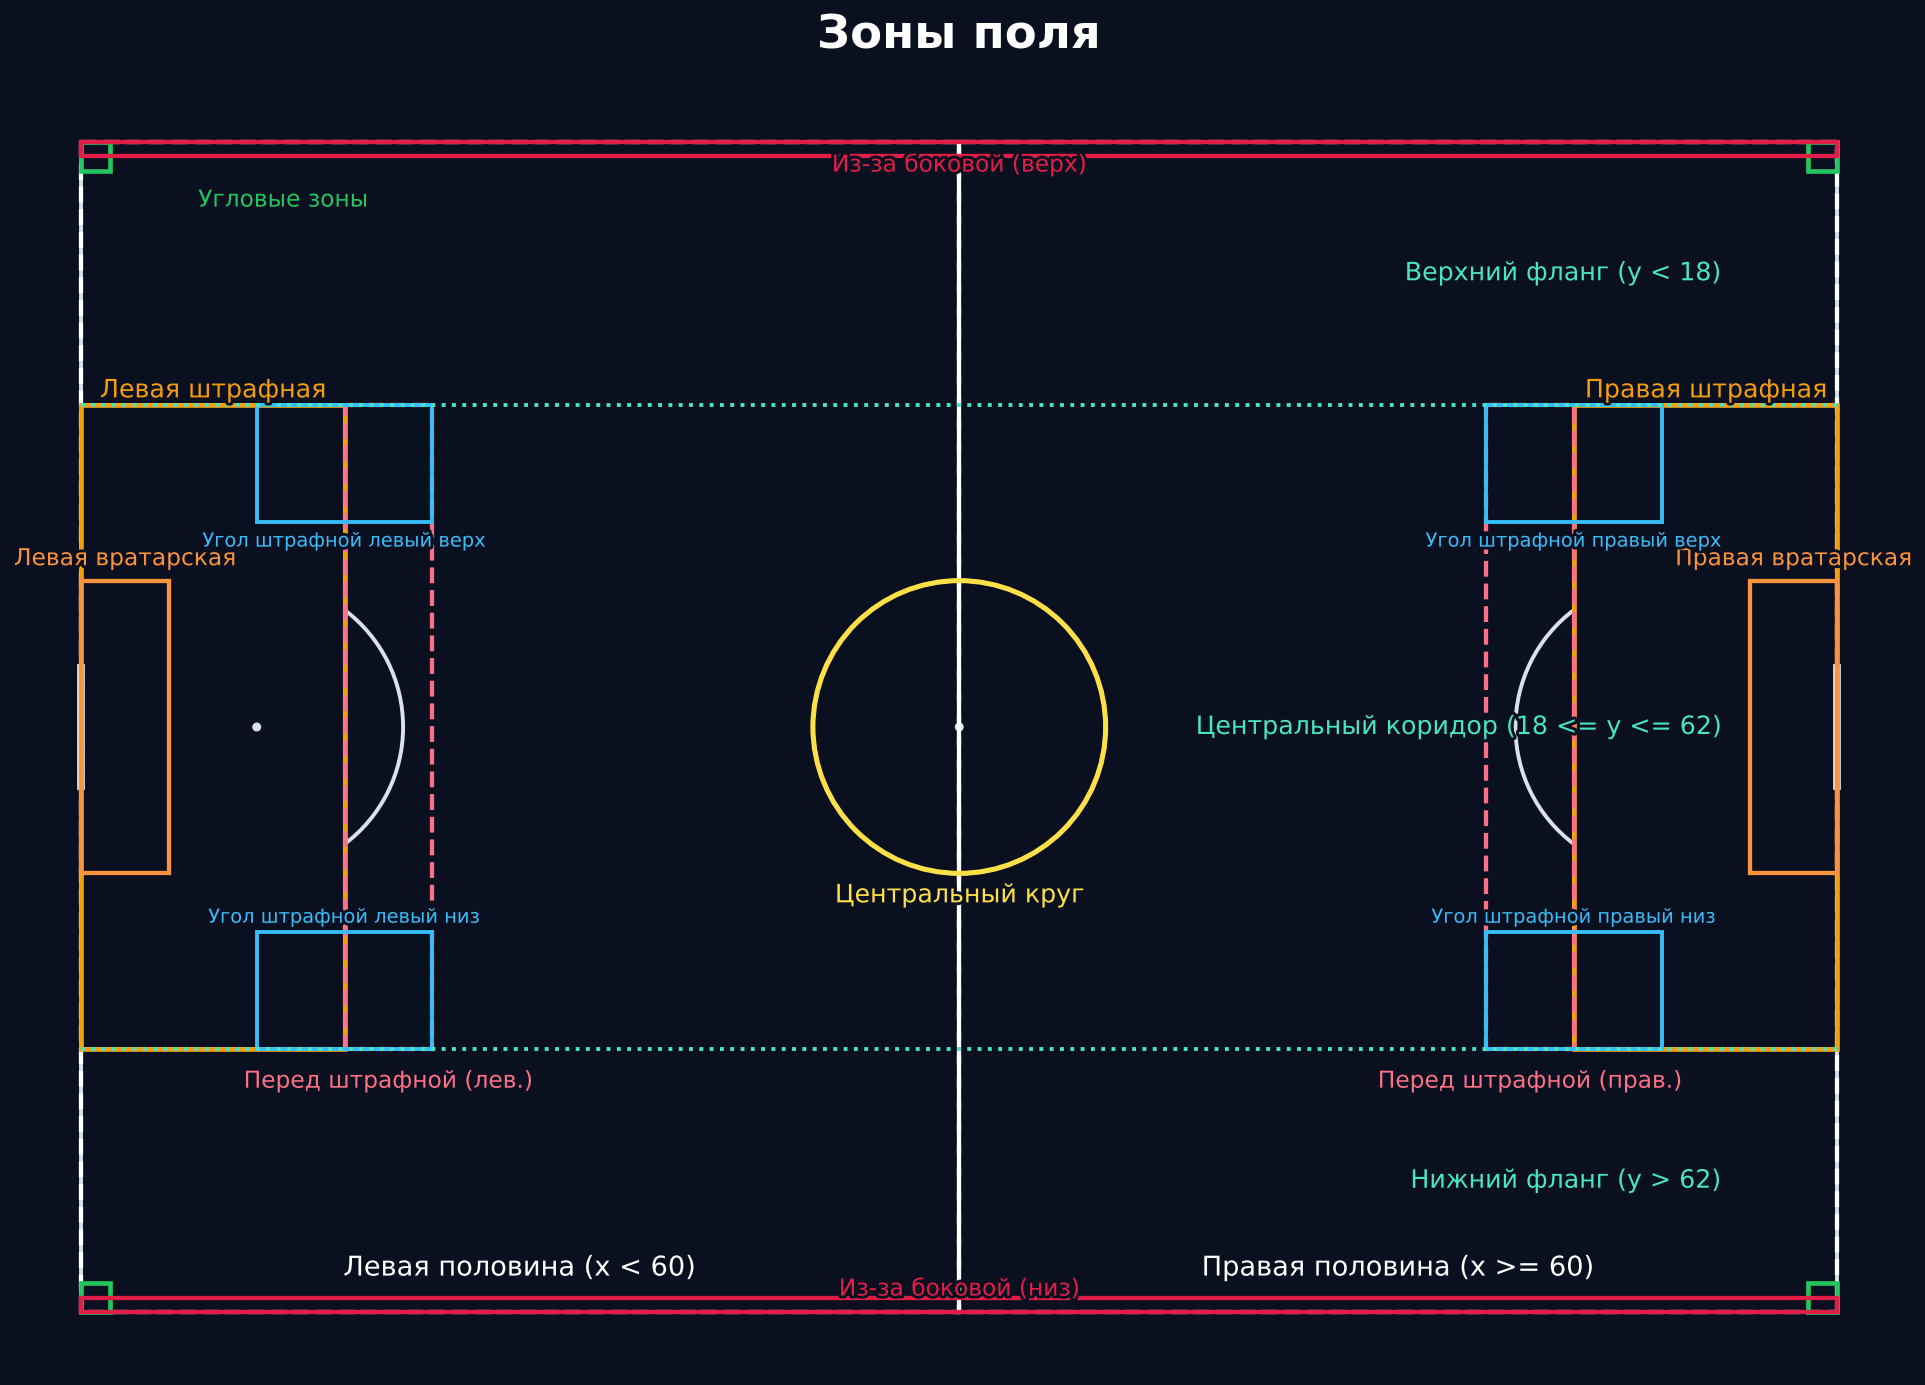
\includegraphics[width=0.92\textwidth]{zones.png}
\caption{Разметка зон поля, используемая для признака \texttt{zone\_label}}
\label{fig:zones}
\end{figure}

\subsection{Фильтрация некорректных 360-кадров}

Для каждого события с StatsBomb~360 проверяется согласованность координаты актёра в freeze-frame и координаты события. Если расстояние между ними превышает порог, 360-контекст для события отключается. Это предотвращает ситуацию, когда визуализация и LLM получают пространственно неверный контекст. На Рисунке~\ref{fig:example-360} показан пример корректной визуализации с 360-контекстом, а на Рисунке~\ref{fig:bad-360} --- пример события, для которого 360-контекст отключается из-за геометрического расхождения.

\begin{figure}[H]
\centering
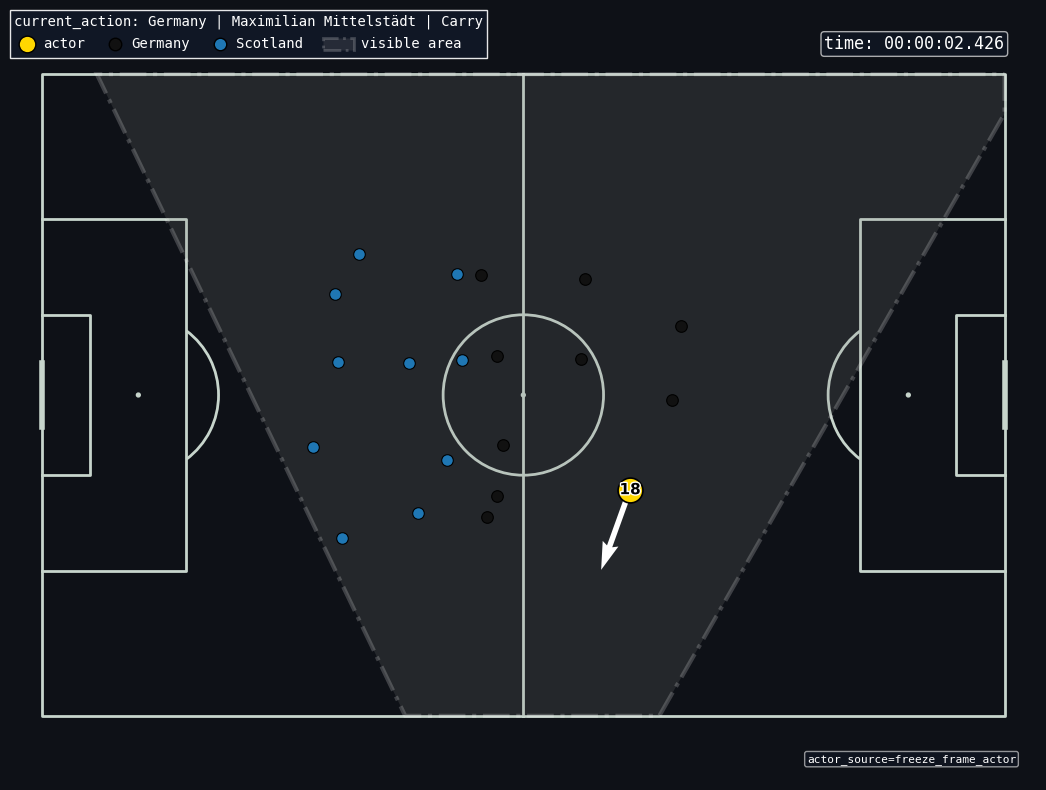
\includegraphics[width=0.82\textwidth]{example_360.png}
\caption{Пример корректной визуализации события с StatsBomb~360}
\label{fig:example-360}
\end{figure}

\begin{figure}[H]
\centering
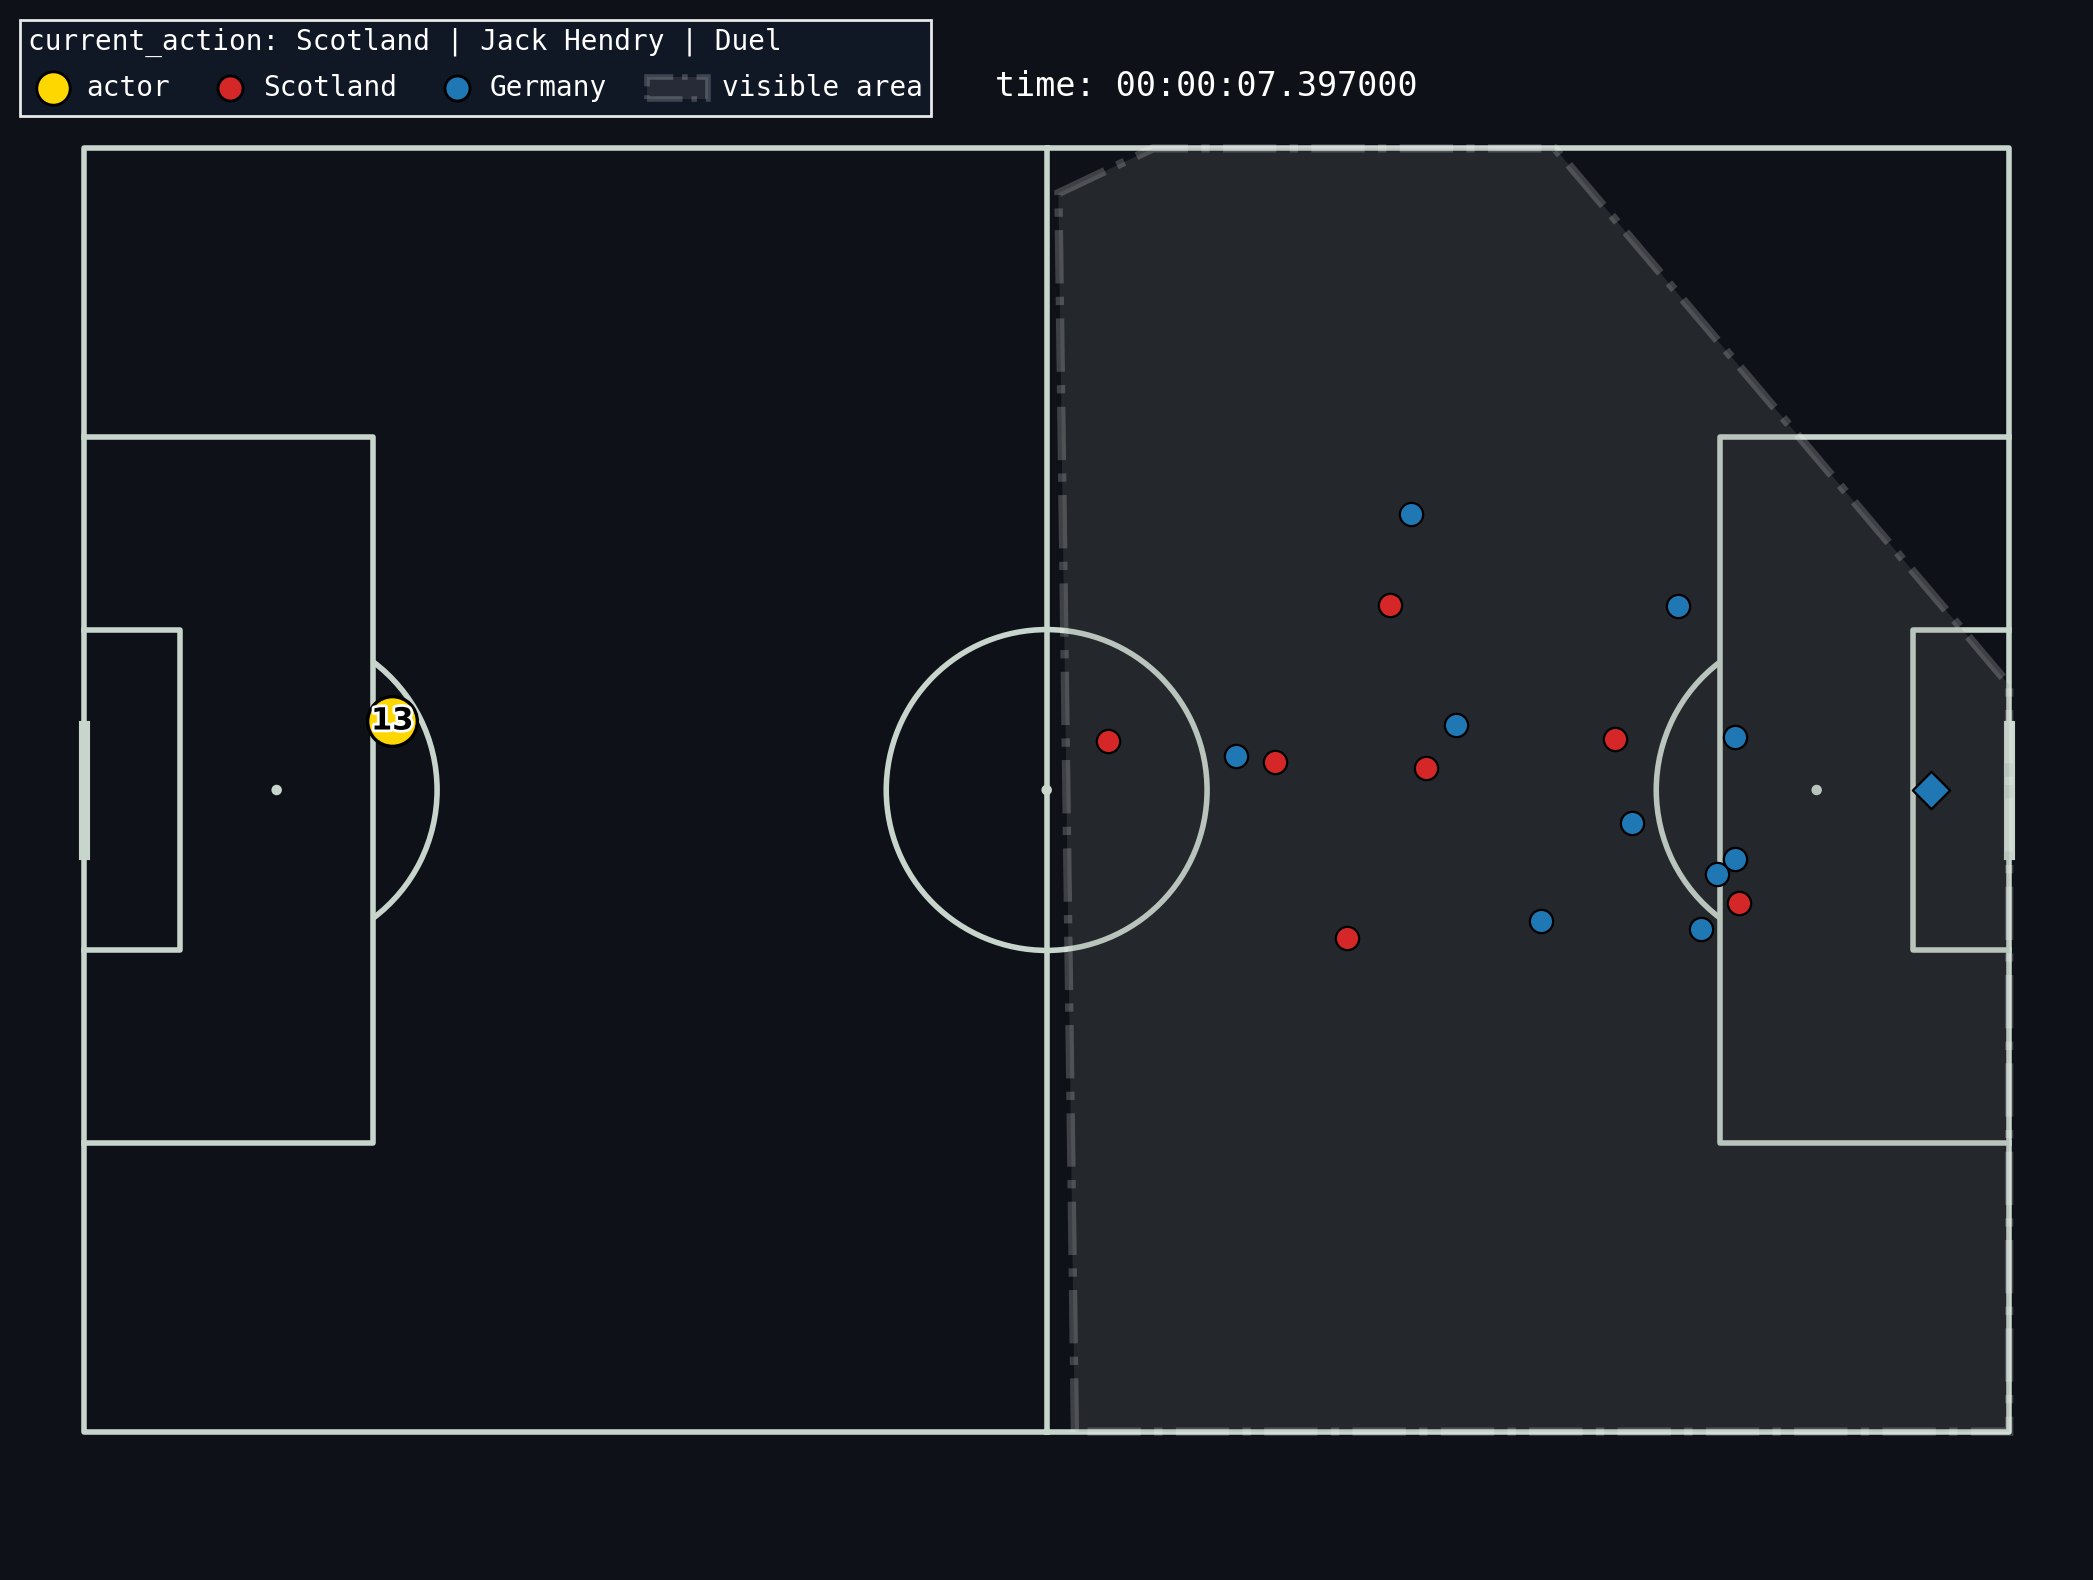
\includegraphics[width=0.88\textwidth]{bad_360.png}
\caption{Пример события с некорректным 360-контекстом, который исключается из payload}
\label{fig:bad-360}
\end{figure}

\subsection{Формирование признаков событий и эпизодов}

После стандартизации координат для каждого события и для каждой цепочки строится расширенное признаковое описание. Оно нужно сразу для двух задач: во-первых, для эвристической soft-разметки важности эпизода; во-вторых, для обучения моделей-селекторов, которые воспроизводят решение о том, нужно ли отправлять эпизод в LLM.

Признаки делятся на несколько групп:

\begin{enumerate}
    \item \textbf{Структурные признаки цепочки}: число событий, длительность, максимальный и средний временной разрыв между соседними событиями, тип первого и последнего события.
    \item \textbf{Игровые признаки значимости}: наличие удара, отбора, перехвата, потери, фола, офсайда, негативного исхода паса, стандарта.
    \item \textbf{Пространственные признаки}: вход на чужую половину, вход в чужую штрафную, выход из своей штрафной, окончание эпизода перед штрафной, у боковой линии или в угловой зоне.
    \item \textbf{Признаки движения}: продвижение к чужим воротам, движение назад, поперечное смещение, прогрессивное ведение, перевод фланга, максимальный и средний прогресс по направлению атаки.
    \item \textbf{Классы событий}: агрегированные счётчики событий разных семантических групп: \texttt{shot}, \texttt{transition}, \texttt{turnover}, \texttt{build\_up}, \texttt{foul}, \texttt{low\_signal}, \texttt{duel}, \texttt{defensive\_action}, \texttt{set\_piece\_or\_ref}, \texttt{meta}, \texttt{discipline}.
\end{enumerate}

Итоговый словарь признаков приведён в Приложении~\ref{app:features}. Такая декомпозиция важна методологически: модель не получает только координаты или только тип события, а видит компактное описание того, насколько эпизод опасен, продвигается ли мяч к воротам, меняется ли зона игры и есть ли в цепочке событие, значимое для комментария.

% =========================
% МЕТОДОЛОГИЯ
% =========================
\section{Методология}\label{sec:methodology}

\subsection{Стратегии формирования эпизодов}

Одно событие StatsBomb не всегда совпадает с тем, что человек воспринимает как футбольный эпизод. Например, передача обычно связана с приёмом мяча, ведением и следующим действием; удар может сопровождаться блоком или действием вратаря; потеря мяча часто имеет смысл только вместе с предыдущей передачей или ведением. Поэтому перед генерацией комментария события нужно объединить в короткие цепочки, которые далее называются эпизодами или payloads.

В работе сравниваются несколько стратегий группировки. Они отвечают на один и тот же вопрос: какие события попадут в один входной JSON для LLM. Сравнение проводится не по качеству текста напрямую, а по промежуточным свойствам эпизодов: сколько payloads получится, насколько длинными они будут, сколько в них значимых событий, как распределятся soft-label классы и насколько устойчиво модель-селектор воспроизводит разметку для такой стратегии. После этого лучшая стратегия используется для финального LLM-прогона.

Базовая идея стратегий семейства \texttt{related} состоит в том, что матч представляется как граф событий. Каждое событие StatsBomb становится вершиной графа. Если в поле \texttt{related\_events} события $e_i$ указан идентификатор события $e_j$, между ними проводится ребро. В реализации ребро рассматривается как неориентированное: если $e_i$ связано с $e_j$, то оба события считаются соседними независимо от направления ссылки. Это важно, потому что в данных StatsBomb связь может быть записана только у одного из двух событий.

После построения графа события просматриваются в хронологическом порядке. Для очередного ещё не использованного события строится связная компонента: берётся само событие, затем все его соседи по \texttt{related\_events}, затем соседи этих соседей и так далее. Полученная компонента сортируется по исходному индексу события в матче и рассматривается как первичная цепочка. Например, передача может быть связана с приёмом мяча, приём --- с ведением, а ведение --- с потерей. Тогда эти четыре события образуют один кандидат в эпизод:

\begin{center}
\texttt{Pass} $\rightarrow$ \texttt{Ball Receipt*} $\rightarrow$ \texttt{Carry} $\rightarrow$ \texttt{Dispossessed}.
\end{center}

Однако связанные компоненты могут быть слишком длинными: особенно в позиционных владениях, где события \texttt{Pass}, \texttt{Ball Receipt*}, \texttt{Carry} и \texttt{Pressure} повторяются много раз подряд. Поэтому для практического использования компоненты дополнительно разбиваются на компактные фрагменты. Для нового события $e_k$ проверяются три условия:

\begin{equation}
\operatorname{cut}(e_k)=1 \quad \Longleftrightarrow \quad
\left(|c| \geq N_{max}\right)
\vee \left(t(e_k)-t(e_{first}) > T_{max}\right)
\vee \left(t(e_k)-t(e_{prev}) > G_{max}\right),
\label{eq:chain-cut}
\end{equation}

где $|c|$ --- число событий в текущем фрагменте, $t(e_{first})$ --- время первого события в нём, $t(e_{prev})$ --- время предыдущего события. Если выполняется хотя бы одно условие, текущий фрагмент завершается, а событие $e_k$ начинает новый фрагмент. Дополнительная стратегия \texttt{related\_stop\_cap} вводит ещё одно правило: если в текущем фрагменте встречается футбольное стоп-событие, например удар, фол, офсайд, потеря, перехват, вынос или действие вратаря, фрагмент также завершается. Такая граница ближе к логике комментария: у эпизода появляется понятный смысловой итог.

\begin{table}[H]
\caption{Стратегии формирования эпизодов из событий StatsBomb}
\label{tab:grouping-strategies}
\centering
\small
\begin{tabular}{p{0.20\textwidth}p{0.34\textwidth}p{0.34\textwidth}}
\toprule
\textbf{Стратегия} & \textbf{Как формируется эпизод} & \textbf{Что проверяет эксперимент} \\
\midrule
\texttt{event\_only} & Каждое событие становится отдельным payload. Цепочек фактически нет. & Базовый вариант: показывает, что произойдёт, если не объединять события. Даёт много коротких входов и высокую стоимость LLM-прогона. \\
\texttt{related\_only} & События объединяются по полю \texttt{related\_events}. Связь рассматривается как двусторонняя: если событие A связано с B, они попадают в один графовый компонент. & Проверяет, достаточно ли встроенных связей StatsBomb для получения смысловых эпизодов. Минус: компоненты могут становиться слишком длинными. \\
\texttt{related\_cap} & Используется тот же граф связанных событий, но цепочка дополнительно режется по максимальному числу событий, длительности и временному разрыву. & Проверяет, помогает ли ограничение длины сделать payload удобнее для LLM и уменьшить риск пересказа слишком длинного фрагмента матча. \\
\texttt{related\_stop\_cap} & К стратегии \texttt{related\_cap} добавляется разрезание по стоп-событиям: удар, фол, офсайд, потеря, перехват, вынос, действие вратаря. & Проверяет гипотезу, что футбольный эпизод должен завершаться на естественной смысловой границе, а не только по техническому лимиту длины. \\
\texttt{time\_window} & События группируются по фиксированным временным окнам без явной опоры на \texttt{related\_events}. & Альтернативный baseline: показывает, насколько хорошо работает простая временная близость без знания связей между событиями. \\
\bottomrule
\end{tabular}
\end{table}

Для ограниченных стратегий используются параметры:

\begin{equation}
    N_{max}=6, \qquad T_{max}=10\text{ секунд}, \qquad G_{max}=4\text{ секунды},
\end{equation}

где $N_{max}$ --- максимальное число событий в эпизоде, $T_{max}$ --- максимальная длительность эпизода, $G_{max}$ --- максимальный допустимый разрыв между соседними событиями. Параметр $G_{max}$ нужен для защиты от склеивания событий, которые формально оказались в одной связанной компоненте, но в реальном времени уже относятся к разным микрофрагментам игры.

Итоговое сравнение стратегий проводится по четырём группам критериев:

\begin{enumerate}
    \item \textbf{Компактность эпизодов}: медианная длина цепочки, квантиль $P_{90}$ по числу событий, средняя и медианная длительность. Длинные цепочки хуже подходят для LLM, потому что модель начинает пересказывать последовательность действий вместо короткого тифлокомментария.
    \item \textbf{Стоимость LLM-прогона}: число payloads, которые придётся отправить в модель. Стратегия \texttt{event\_only} обычно создаёт слишком много входов, а \texttt{related\_only} может создавать слишком длинные входы.
    \item \textbf{Распределение soft-labels}: доля классов \texttt{skip}, \texttt{brief}, \texttt{must}. Это показывает, какая часть сформированных эпизодов потенциально требует озвучивания.
    \item \textbf{Качество селектора}: macro-F1, weighted-F1, balanced accuracy и accuracy при предсказании \texttt{soft\_label\_3}. Эти метрики показывают, насколько стабильно признаки эпизода позволяют воспроизвести выбранную методологию отбора.
\end{enumerate}

Таким образом, сравнение стратегий --- это сравнение разных способов подготовить вход для LLM. В финальный генеративный этап не отправляется весь поток событий: сначала выбирается стратегия группировки, затем для полученных эпизодов считается soft-label, после чего в LLM отправляются только эпизоды классов \texttt{brief} и \texttt{must}.

\subsection{Soft-разметка важности эпизодов}

Готовой ручной разметки того, какие эпизоды футбольного матча нужно озвучивать, в данных нет. Поэтому в работе используется weak supervision: целевая переменная задаётся не экспертной разметкой, а прозрачной эвристикой, построенной на футбольных признаках. Такая разметка называется soft-label, потому что она не является абсолютной истиной, но задаёт согласованное приближение к задаче отбора эпизодов.

Эвристики формировались не только по структуре StatsBomb JSON. Перед фиксацией правил вручную просматривались и анализировались футбольные трансляции Okko с точки зрения того, какие действия комментатор описывает в первую очередь, как часто называется положение мяча, как проговариваются передачи, стандарты, потери, удары и игровые паузы. Этот ручной просмотр использовался как практический ориентир для правил тифлокомментария: комментарий должен быстро отвечать на вопросы «где мяч?», «кто действует?», «что произошло?» и «чем завершился эпизод?». Поэтому в эвристику попали не все события подряд, а именно те, которые создают смысловой итог для слушателя: удары, входы в штрафную, продвижение к воротам, длинные передачи, переводы фланга, перехваты, потери, фолы, офсайды и стандарты. Низкосигнальные события вроде простого приёма мяча или давления без исхода, наоборот, не должны перегружать аудиодорожку.

Для эпизода $c$ вычисляется одно числовое значение важности $S(c)$:

\begin{equation}
\begin{split}
S(c) ={}& 3.0 \cdot n_{shot} + 2.5 \cdot n_{box} + 2.0 \cdot n_{high} + 1.5 \cdot n_{longpass} \\
&+ 1.2 \cdot n_{forward} + 1.2 \cdot n_{switch} + 1.0 \cdot n_{badpass} + 0.8 \cdot n_{setplay} \\
&- 0.35 \cdot n_{low} - P(c).
\end{split}
\label{eq:soft-score}
\end{equation}

Здесь все $n_{\cdot}$ --- неотрицательные целочисленные счётчики событий внутри эпизода $c$: $n_{shot}$ --- число ударов, $n_{box}$ --- число входов в чужую штрафную, $n_{high}$ --- число событий высокой значимости, $n_{longpass}$ --- число длинных передач, $n_{forward}$ --- число продвижений вперёд, $n_{switch}$ --- число переводов фланга, $n_{badpass}$ --- число неудачных передач, $n_{setplay}$ --- число стандартов, $n_{low}$ --- число низкосигнальных событий. Чем длиннее эпизод и чем больше в нём футбольных действий, тем больше потенциальное значение $S(c)$; сверху оно специально не ограничивается, потому что эпизоды могут содержать разное число событий. Снизу score также может быть отрицательным: это означает, что в эпизоде преобладают низкосигнальные или технические действия, которые не нужно озвучивать отдельно.

Отдельный штраф $P(c)$ задаётся как
\begin{equation}
P(c) = 2 \cdot \mathbb{I}\{N(c)=1,\ n_{low}=1\} + 0.5 \cdot \mathbb{I}\{T(c)>15,\ n_{shot}=0\},
\label{eq:soft-penalty}
\end{equation}
где $N(c)$ --- число событий в цепочке, $T(c)$ --- длительность цепочки в секундах, а $\mathbb{I}\{\cdot\}$ --- индикатор условия, равный $1$, если условие выполнено, и $0$ иначе. Поэтому $P(c)$ может принимать значения $0$, $0.5$, $2$ или $2.5$. Первый штраф убирает одиночные низкосигнальные события, например отдельный приём мяча или давление без исхода. Второй штраф снижает важность слишком длинных неопасных цепочек: если эпизод длится больше 15 секунд и в нём нет удара, он не должен автоматически становиться важным только из-за длины.

Положительные слагаемые в формуле~\eqref{eq:soft-score} повышают важность эпизода, потому что они соответствуют действиям, которые помогают слушателю понять развитие матча: удар, вход в штрафную, продвижение к воротам, длинная передача, перевод фланга, стандарт или явный неудачный исход. Отрицательные слагаемые нужны для обратной задачи --- не перегружать аудиодорожку событиями, которые сами по себе мало что меняют. Поэтому формула одновременно решает две задачи: поднимает приоритет содержательных эпизодов и понижает приоритет технических или слишком растянутых цепочек без опасного итога.

Эта формула не претендует на роль истинной экспертной разметки. Её задача другая: зафиксировать явные футбольные правила в воспроизводимом виде и получить proxy-метки для большого числа эпизодов. Поэтому веса задаются не обучением, а экспертной логикой: сначала выделяются действия, которые в реальном комментарии почти нельзя пропустить, затем действия, которые важны только в контексте развития атаки, и, наконец, низкосигнальные события, которые сами по себе не должны перегружать аудиодорожку. Такой подход позволяет прозрачно объяснить, почему эпизод попал или не попал в LLM.

Содержательно веса можно разделить на три уровня. Вес $3.0$ для удара означает событие максимального приоритета: удар почти всегда должен быть озвучен. Вес $2.5$ для входа в штрафную отражает рост опасности эпизода даже без удара. Веса $1.0$--$1.5$ соответствуют развитию атаки: длинная передача, продвижение вперёд, перевод фланга или неудачный исход паса. Отрицательный вес для $n_{low}$ и штраф $P(c)$ нужны, чтобы цепочки из приёмов мяча и давления без результата не получали высокий приоритет только из-за длины.

Промежуточная пятибалльная шкала $y_5$ задаётся по порогам score:

\begin{equation}
 y_5(c) =
 \begin{cases}
 0, & S(c) \le 0,\\
 1, & 0 < S(c) \le 1.5,\\
 2, & 1.5 < S(c) \le 3.5,\\
 3, & 3.5 < S(c) \le 6.0,\\
 4, & S(c) > 6.0.
 \end{cases}
\end{equation}

Содержательно классы интерпретируются так:

\begin{table}[H]
\caption{Интерпретация пяти классов эвристической важности}
\label{tab:soft-label-5}
\centering
\small
\begin{tabular}{p{0.10\textwidth}p{0.27\textwidth}p{0.52\textwidth}}
\toprule
\textbf{Класс} & \textbf{Название} & \textbf{Смысл} \\
\midrule
0 & шумовой эпизод & Служебное или низкосигнальное действие, которое не нужно озвучивать отдельно. \\
1 & слабый сигнал & Есть минимальное футбольное действие, но без заметного продвижения или исхода. Обычно не отправляется в LLM. \\
2 & умеренный эпизод & Есть развитие владения, переход зоны или действие, которое можно кратко прокомментировать. \\
3 & значимый эпизод & Есть заметное продвижение, стандарт, потеря, перехват или другой смысловой итог. Желательно прокомментировать. \\
4 & обязательный эпизод & Удар, опасная доставка, вход в штрафную, важный исход или комбинация нескольких сильных признаков. Обязательно отправляется в генерацию. \\
\bottomrule
\end{tabular}
\end{table}

Для практического селектора пятибалльная шкала агрегируется в три класса:

\begin{equation}
 y_3(c) =
 \begin{cases}
 0, & y_5(c) \in \{0,1\} \quad \text{не комментировать},\\
 1, & y_5(c) \in \{2,3\} \quad \text{кратко прокомментировать},\\
 2, & y_5(c)=4 \quad \text{обязательно комментировать}.
 \end{cases}
\end{equation}

Именно $y_3$ используется как основная целевая переменная для моделей отбора и для формирования финальных payloads в LLM: класс 0 отбрасывается, класс 1 получает режим \texttt{brief}, класс 2 --- режим \texttt{must}.

Таким образом, задача моделей отбора формулируется не как обучение «идеальному комментатору», а как обучение селектору, который приближает заданную методологию отбора эпизодов. Это важно для интерпретации результатов: высокое качество на полном наборе признаков означает, что модель научилась воспроизводить эвристическую разметку, а не доказывает абсолютное качество комментария. Поэтому дополнительно анализируется сокращённый набор признаков без прямых членов формулы и проводится отдельная оценка LLM-ответов.

\subsection{Модели отбора эпизодов}

Логистическая регрессия и CatBoost в данной работе используются не как самостоятельные генераторы комментариев. Их роль более узкая: это модели-селекторы, которые по признакам эпизода предсказывают, нужно ли отправлять этот эпизод в LLM и в каком режиме: не комментировать, кратко прокомментировать или обязательно прокомментировать. Иными словами, LLM отвечает за текст, а классическая модель отвечает за предварительный отбор эпизодов.

На первый взгляд может показаться, что обучение модели избыточно, поскольку soft-label уже задаётся формулой. Однако формула в этой работе играет роль первичной разметки, а не конечного продукта. Она нужна, чтобы получить воспроизводимые proxy-метки на большом наборе матчей без ручной разметки каждого эпизода. Модели отбора проверяют, можно ли автоматизировать это решение по признаковому описанию эпизода и насколько это описание переносимо между матчами. В дальнейшем та же схема может быть использована с ручной или смешанной разметкой: формула задаёт стартовые метки, а модель дообучается на экспертных оценках.

Такое разделение нужно по двум причинам. Во-первых, отправлять в LLM все события матча дорого и неэффективно: большая часть событий является низкосигнальной и не требует отдельного комментария. Во-вторых, модель-селектор позволяет отделить задачу отбора от задачи генерации. Это делает пайплайн управляемым: можно менять стратегию группировки, порог отбора, набор признаков и модель селектора, не переписывая промпт и не перегружая LLM лишними событиями.

Логистическая регрессия выбрана как простая линейная базовая модель. Она показывает, насколько задача решается почти линейной комбинацией признаков. CatBoost выбран как более сильная модель для табличных данных: он умеет работать с категориальными признаками, нелинейными взаимодействиями и неоднородными числовыми шкалами. Сравнение этих моделей позволяет понять, есть ли в признаках полезные нелинейные зависимости или достаточно простой линейной схемы.

Перед обучением каждый эпизод переводится в одну строку табличного датасета. Это принципиальный момент: модели не получают полный JSON матча и не генерируют текст. Они получают только агрегированные признаки эпизода и предсказывают класс важности \texttt{soft\_label\_3}. Формат входа для моделей приведён в Таблице~\ref{tab:selector-training-data}.

\begin{table}[H]
\centering
\small
\caption{Что передавалось в модели отбора CatBoost и LogReg}
\label{tab:selector-training-data}
\begin{tabular}{p{0.24\textwidth}p{0.66\textwidth}}
\toprule
\textbf{Компонент} & \textbf{Описание} \\
\midrule
Наблюдение & Одна строка соответствует одному сформированному эпизоду, то есть одному payload после группировки событий. В основном эксперименте используется стратегия \texttt{related\_stop\_cap}. \\
Целевая переменная & \texttt{soft\_label\_3}: 0 --- не комментировать, 1 --- кратко прокомментировать, 2 --- обязательно прокомментировать. Метка получается из эвристической пятибалльной шкалы \texttt{soft\_label\_5}. \\
Числовые признаки & Длина и длительность эпизода, временные разрывы, счётчики классов событий, признаки стандартов, ударов, потерь, продвижения мяча, входа в чужую половину и штрафную, переводов фланга, негативных исходов передач и пространственных переходов. \\
Категориальные признаки & Тип первого и последнего события, тайм, стадия турнира, начальные и конечные относительные зоны, доминирующий переход зоны и другие дискретные описания структуры эпизода. \\
Что не передавалось & Сырые JSON целиком, текст комментария, ответ LLM, идентификаторы событий как самостоятельные признаки и целевые поля. В честных режимах также исключались прямые компоненты формулы score. \\
Разбиение & Train/validation/test формируются по \texttt{match\_id}, чтобы события одного матча не попадали одновременно в обучение и тест. Это снижает риск утечки между соседними эпизодами одного матча. \\
Предобработка & Для LogReg числовые признаки масштабируются, категориальные кодируются. CatBoost получает числовые признаки и категориальные столбцы напрямую через механизм \texttt{cat\_features}. \\
\bottomrule
\end{tabular}
\end{table}


При этом важно избежать самообмана. Поскольку soft-label строится по формуле~\eqref{eq:soft-score}, часть признаков одновременно участвует и в разметке, и во входе модели. Если обучать модель на полном наборе признаков, она почти напрямую восстанавливает формулу. Поэтому в эксперименте отдельно проверяется не только «может ли модель повторить формулу», но и «остаётся ли сигнал, если убрать прямые компоненты этой формулы». Для этого используются три набора признаков:

\begin{enumerate}
    \item \texttt{full} --- все признаки, включая прямые компоненты формулы score. Этот режим нужен как sanity check: модель должна уметь воспроизвести заданную эвристику.
    \item \texttt{no\_exact\_score\_terms} --- из входа убираются прямые компоненты формулы score: \texttt{class\_shot\_n}, \texttt{entered\_opp\_box\_n}, \texttt{high\_event\_n}, \texttt{long\_pass\_n}, \texttt{forward\_moves\_n}, \texttt{switched\_flank\_n}, \texttt{bad\_pass\_outcome\_n}, \texttt{set\_play\_n}, \texttt{low\_signal\_n}, а также \texttt{events\_n} и \texttt{duration\_sec}, которые входят в штрафы. Этот режим показывает, можно ли приблизить решение по косвенным признакам.
    \item \texttt{structure\_zone\_only} --- остаются в основном структура эпизода, зоны, движение и типы первого/последнего события. Это всё ещё не gold-оценка, но такой набор меньше похож на прямое восстановление формулы и лучше показывает информативность пространственно-структурного описания.
\end{enumerate}

Таким образом, результаты моделей не трактуются как доказательство «истинной» важности эпизодов. Они показывают, насколько предложенная soft-разметка воспроизводима по признакам и насколько выбранное признаковое описание достаточно информативно для автоматического селектора. Главная интерпретационная ценность здесь не в почти единичном качестве на \texttt{full}, а в сравнении с \texttt{no\_exact\_score\_terms} и \texttt{structure\_zone\_only}: именно эти режимы показывают, сохраняется ли полезная информация после удаления прямых членов эвристики.

% =========================
% ЭКСПЕРИМЕНТЫ
% =========================
\section{Эксперименты и результаты}\label{sec:experiments}

\subsection{Сравнение стратегий группировки}

\begin{figure}[H]
\centering
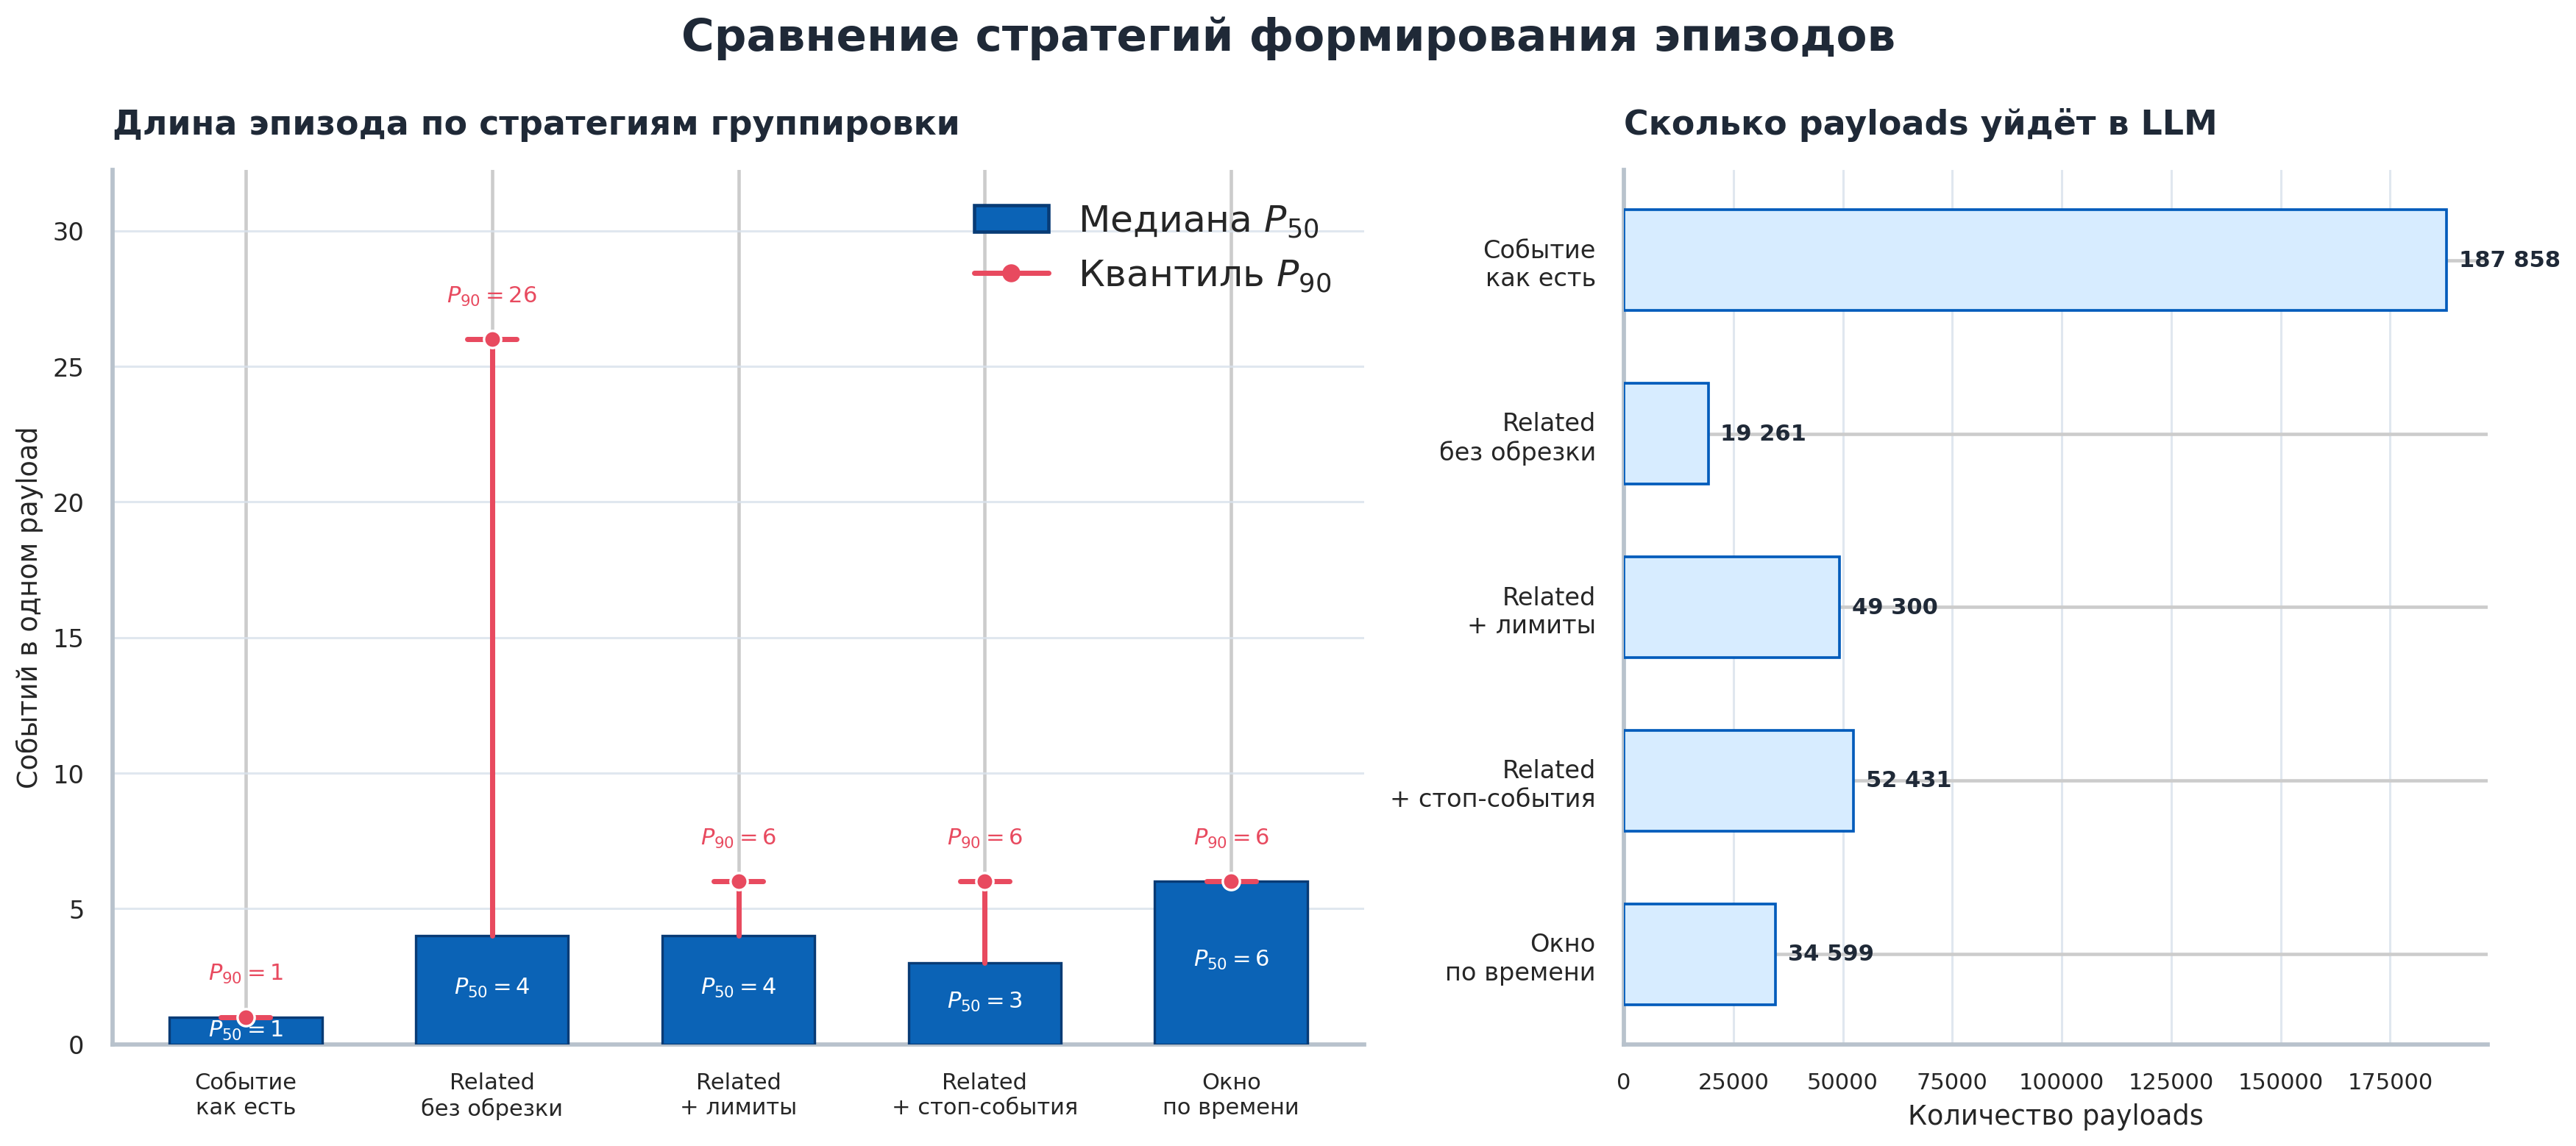
\includegraphics[width=0.98\textwidth]{grouping_strategy_compactness.png}
\caption{Сравнение стратегий формирования эпизодов по длине цепочек и числу payloads на всех матчах Евро-2024}
\label{fig:grouping-compactness}
\end{figure}

\begin{figure}[H]
\centering
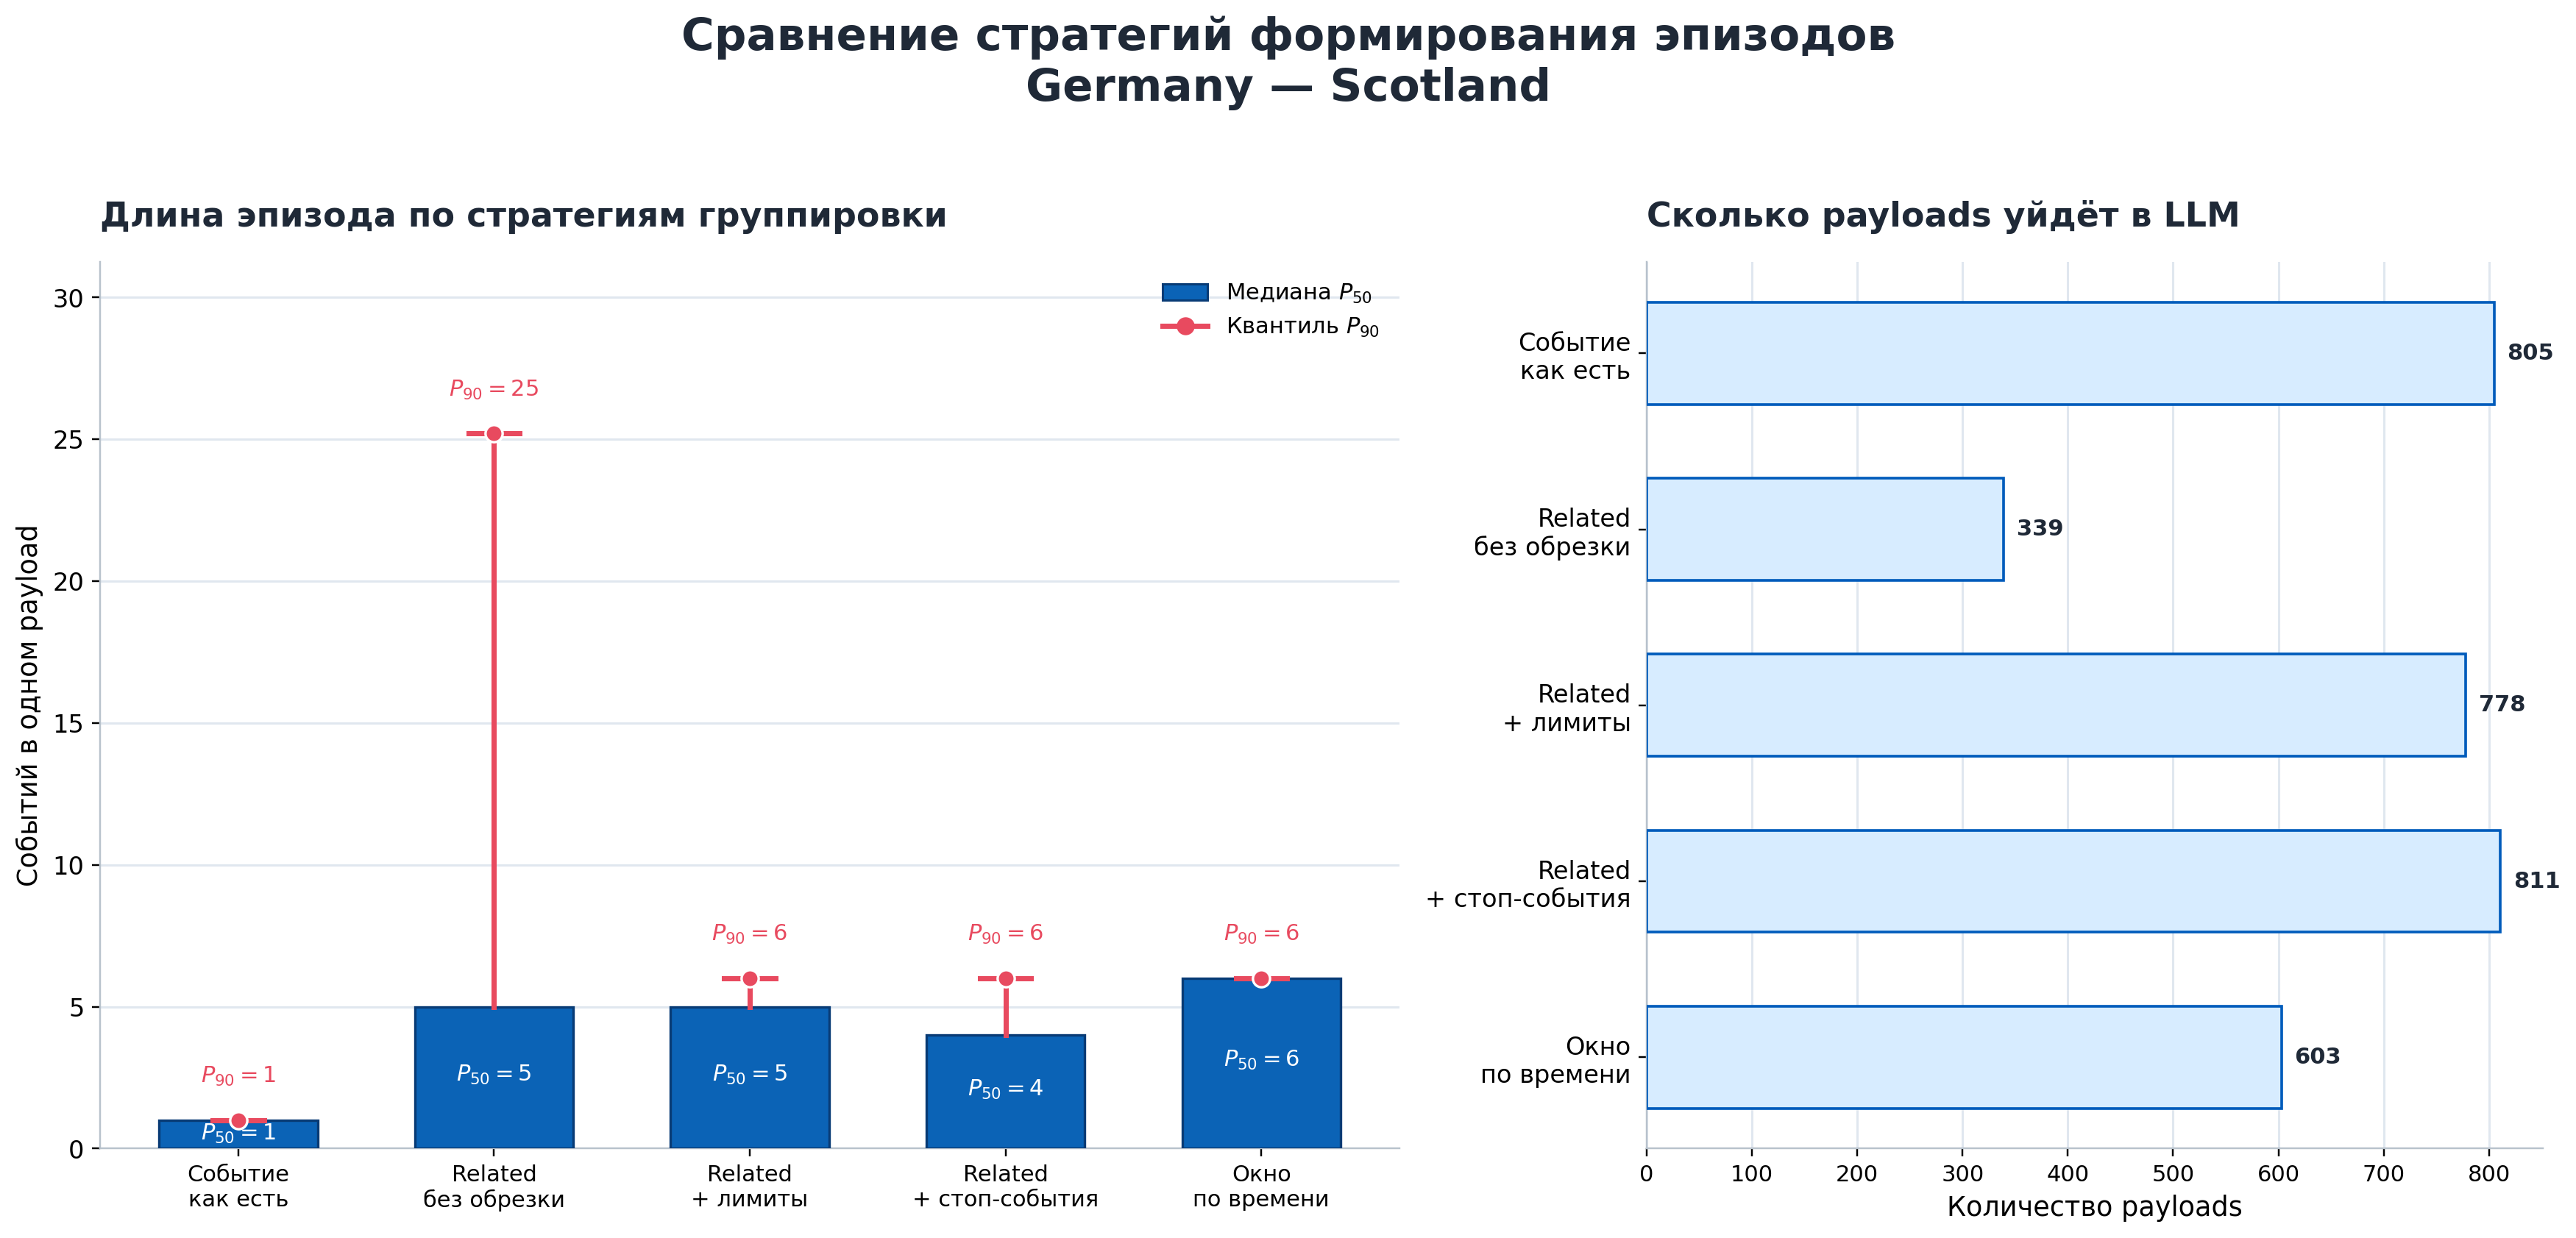
\includegraphics[width=0.98\textwidth]{germany_scotland_grouping_strategy_compactness.png}
\caption{Сравнение стратегий формирования эпизодов для матча Германия --- Шотландия}
\label{fig:grouping-compactness-germany-scotland}
\end{figure}

Основной вывод сравнения: стратегия \texttt{related\_stop\_cap} сохраняет связность событий через \texttt{related\_events}, но дополнительно ограничивает длину цепочки и завершает эпизод на естественных смысловых границах. Поэтому она выбрана как основная стратегия для финального LLM-прогона.

\begin{table}[H]
\centering
\small
\caption{Сравнение стратегий группировки и экспертная оценка качества комментариев}
\label{tab:llm-strategy-quality}
\begin{threeparttable}
\begin{tabular}{lrrrr}
\toprule
\textbf{Стратегия} & \textbf{Payloads для LLM} & \textbf{$P_{50}$ событий} & \textbf{$P_{90}$ событий} & \textbf{Оценка 1--5} \\
\midrule
\texttt{event\_only} & 6056 & 1 & 1 & 2 \\
\texttt{related\_only} & 1977 & 4 & 26 & 3 \\
\texttt{related\_cap} & 5307 & 4 & 6 & 4 \\
\texttt{related\_stop\_cap} & 5604 & 3 & 6 & \textbf{5} \\
\texttt{time\_window} & 4163 & 6 & 6 & 3 \\
\bottomrule
\end{tabular}
\begin{tablenotes}\footnotesize
\item Payloads для LLM посчитаны для набора матчей, выбранных для озвучивания, после фильтрации класса \texttt{skip}. $P_{50}$ и $P_{90}$ характеризуют длину payloads внутри соответствующей стратегии.
\item Оценка 1--5 выставлена по ручному просмотру качества комментариев: 1 --- непригодно, 5 --- наиболее пригодно для финальной озвучки. Отдельный детальный пример для матча Германия --- Шотландия показан на Рисунке~\ref{fig:grouping-compactness-germany-scotland}.
\end{tablenotes}
\end{threeparttable}
\end{table}


Таблица~\ref{tab:llm-strategy-quality} показывает технические характеристики стратегий и итоговую экспертную оценку качества комментариев. Число payloads относится к набору матчей, отобранных для озвучивания, а квантили $P_{50}$ и $P_{90}$ показывают типичную длину и хвост длинных цепочек внутри стратегии. Отдельно для матча Германия --- Шотландия был построен график на Рисунке~\ref{fig:grouping-compactness-germany-scotland}; он использовался как подробный ручной sanity-check выбранной стратегии. Вариант \texttt{event\_only} оказался слишком атомарным: модель часто комментировала отдельное действие без достаточного контекста, поэтому реплики звучали фрагментарно. В \texttt{related\_only} появлялся контекст, но длинный хвост цепочек приводил к пересказу последовательности действий и словам-связкам вроде «затем» или «после этого». Стратегия \texttt{time\_window} давала ровные по длине фрагменты, но иногда объединяла независимые действия или разрывала связанные события. \texttt{related\_cap} заметно улучшала стабильность за счёт ограничений длины, однако граница эпизода не всегда совпадала с футбольным итогом. Поэтому итоговой выбрана \texttt{related\_stop\_cap}: она сохраняет связанные события, ограничивает длину payload и завершает цепочку на смысловой границе --- ударе, фоле, офсайде, потере, перехвате, выносе или действии вратаря.

\subsection{Распределение soft-labels}

\begin{figure}[H]
\centering
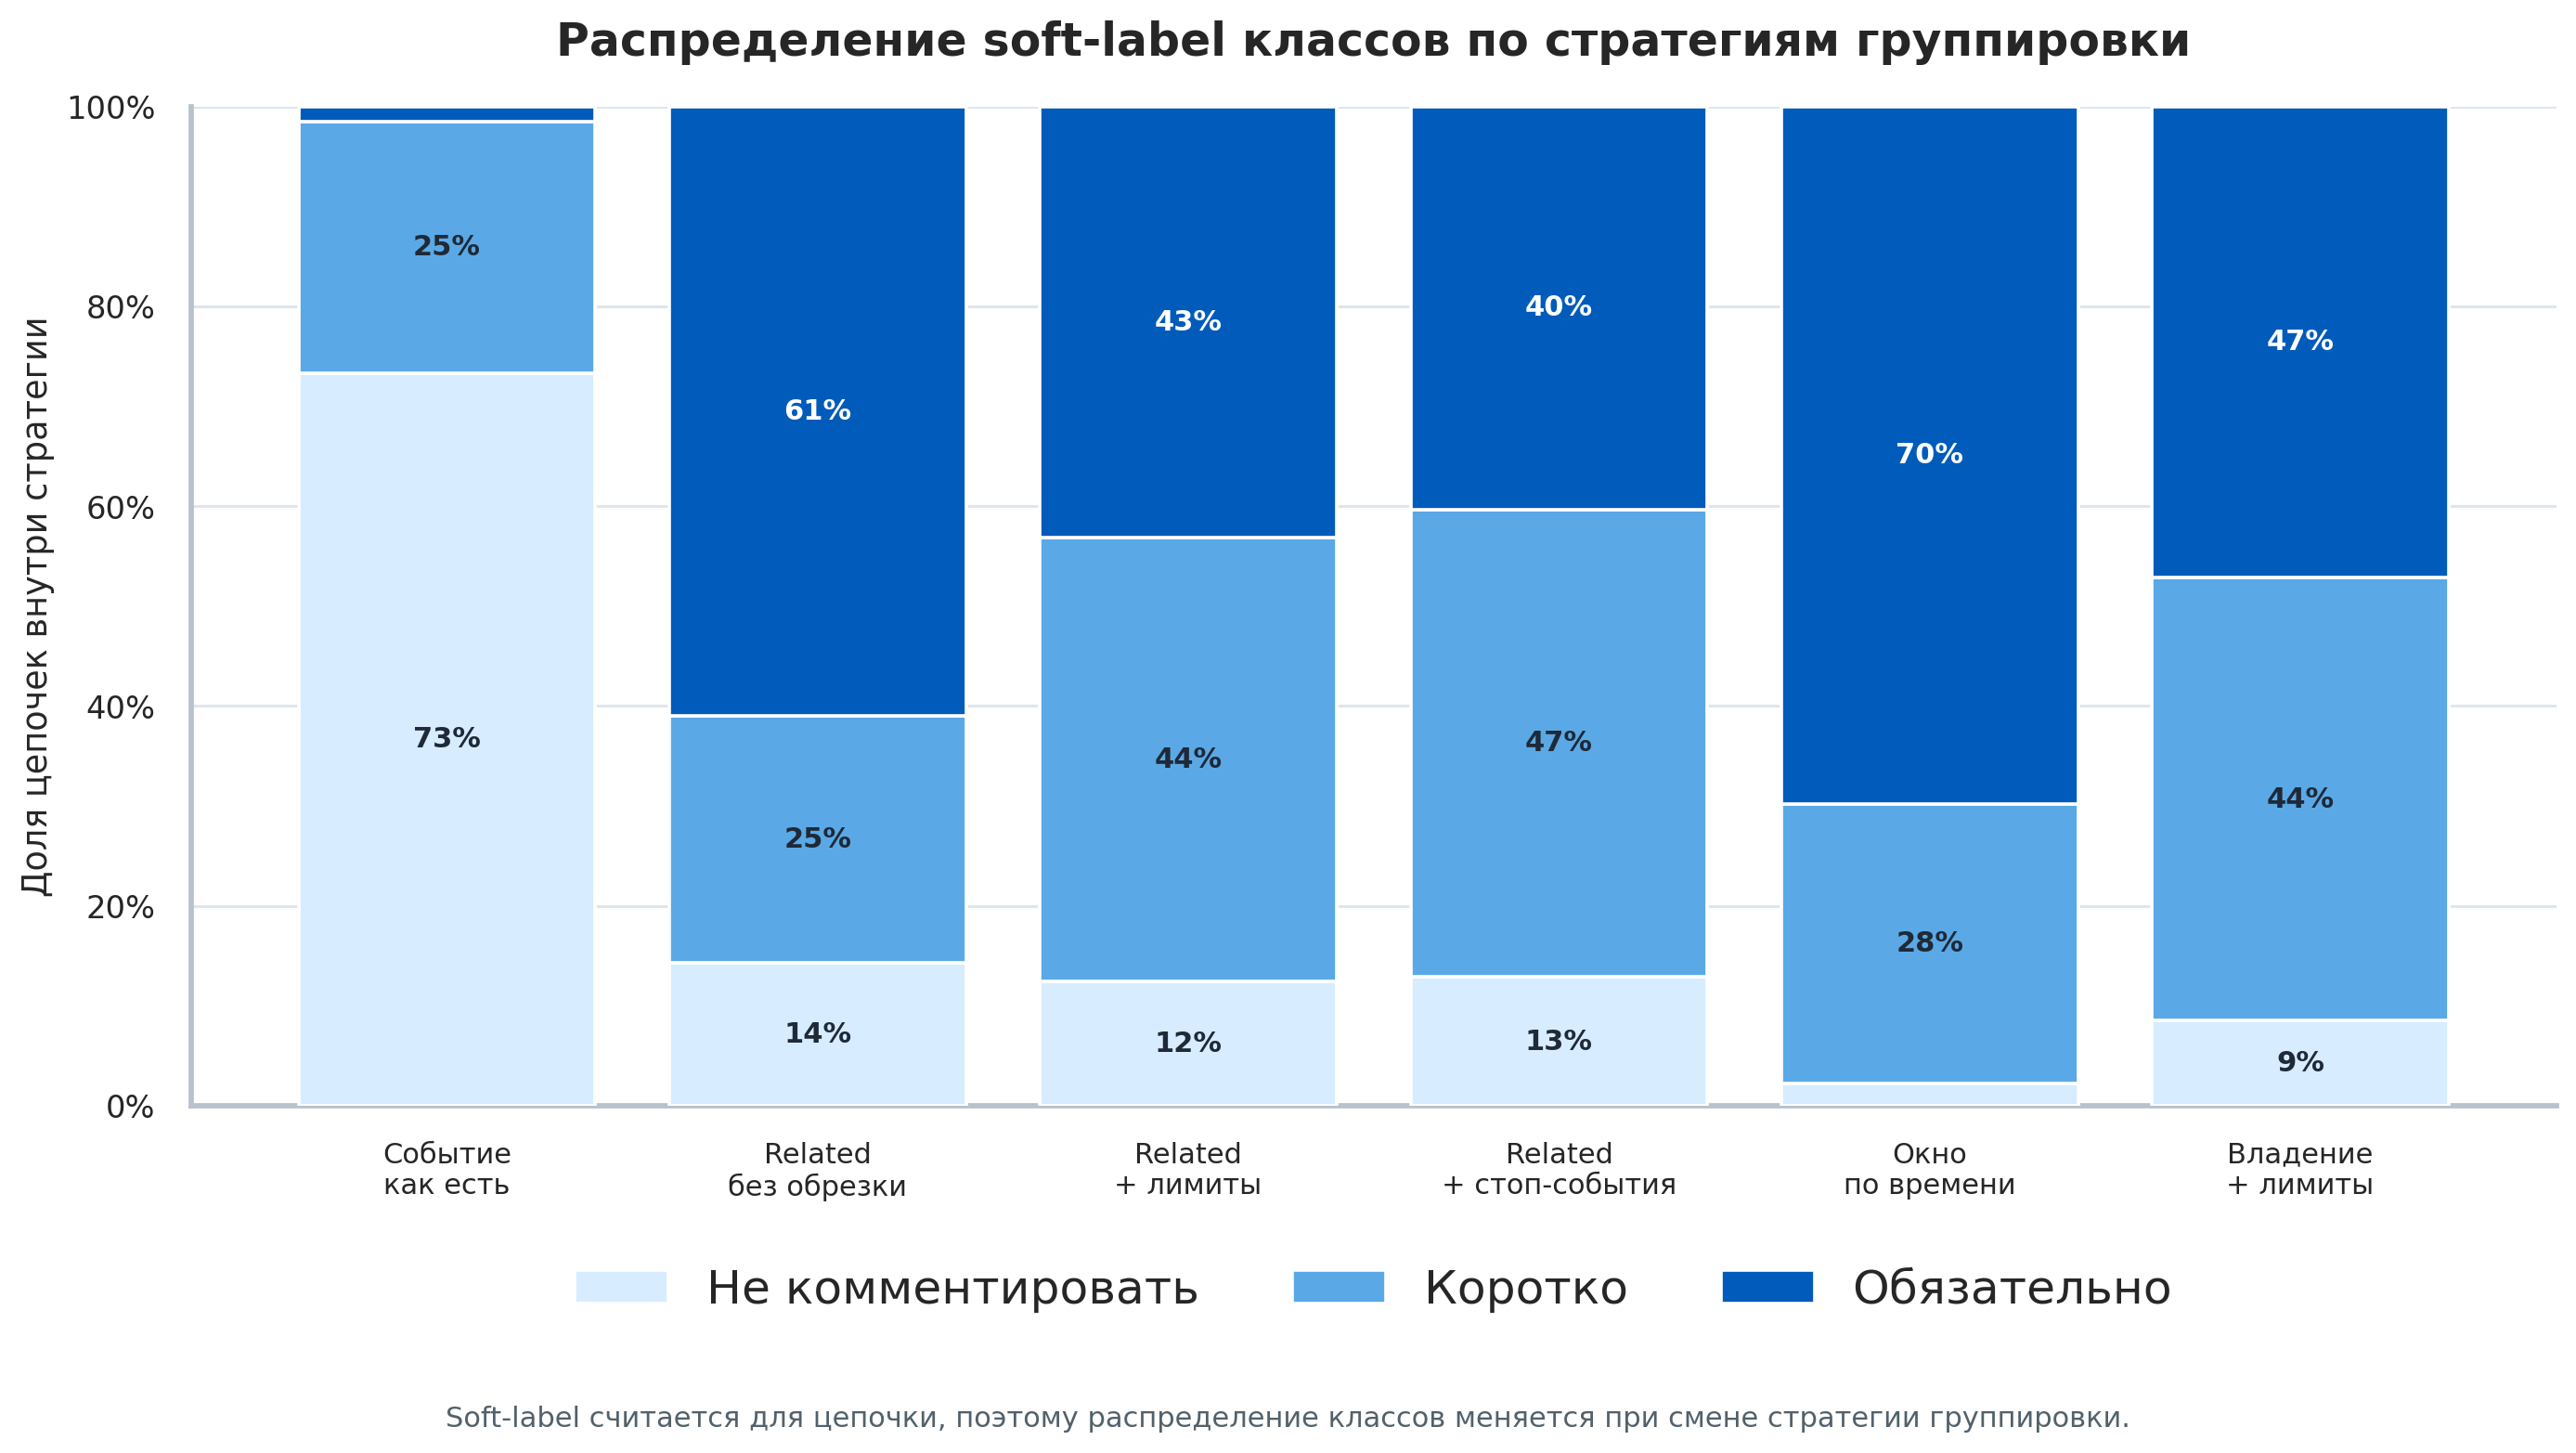
\includegraphics[width=0.92\textwidth]{soft_label_3_distribution_by_strategy.png}
\caption{Распределение классов \texttt{soft\_label\_3} по стратегиям группировки}
\label{fig:soft-label-strategy}
\end{figure}

Распределение классов зависит от стратегии группировки, поскольку soft-label назначается не отдельному событию, а эпизоду. Например, \texttt{event\_only} создаёт много коротких низкосигнальных элементов, тогда как \texttt{related\_only} формирует более длинные цепочки с большим числом значимых действий.

\subsection{Качество моделей отбора}

После сравнения стратегий группировки для основного эксперимента с моделями фиксируется стратегия \texttt{related\_stop\_cap}. Это сделано намеренно: иначе в одном сравнении смешивались бы две разные задачи --- выбор способа группировки событий и качество модели-селектора. Сначала выбирается способ получить эпизод, затем уже на эпизодах одной структуры сравниваются признаки и модели, предсказывающие \texttt{soft\_label\_3}.

Для оценки используются accuracy, macro-F1, weighted-F1 и balanced accuracy. Основной метрикой выбрана macro-F1, поскольку классы несбалансированы, а ошибки на редком классе \texttt{must} особенно важны для качества озвучки. Accuracy в такой задаче может быть завышена за счёт частого класса, тогда как macro-F1 усредняет качество по классам равномерно.

\begin{table}[H]
\centering
\small
\caption{Качество моделей отбора эпизодов для разных наборов признаков}
\label{tab:model-results}
\begin{threeparttable}
\begin{tabular}{llcrrrr}
\toprule
Набор признаков & Модель & Split & Macro-F1 & Weighted-F1 & Balanced Acc. & Accuracy \\
\midrule
\texttt{full} & LogReg & val & 0.999 & 0.999 & 0.999 & 0.999 \\
\texttt{full} & LogReg & test & 0.999 & 0.999 & 0.999 & 0.999 \\
\texttt{full} & CatBoost & val & 0.999 & 1.000 & 0.999 & 1.000 \\
\texttt{full} & CatBoost & test & 1.000 & 1.000 & 1.000 & 1.000 \\
\texttt{no\_exact\_score\_terms} & LogReg & val & 0.813 & 0.820 & 0.822 & 0.822 \\
\texttt{no\_exact\_score\_terms} & LogReg & test & 0.815 & 0.821 & 0.823 & 0.823 \\
\texttt{no\_exact\_score\_terms} & CatBoost & val & 0.846 & 0.854 & 0.853 & 0.854 \\
\texttt{no\_exact\_score\_terms} & CatBoost & test & 0.848 & 0.856 & 0.855 & 0.856 \\
\texttt{structure\_zone\_only} & LogReg & val & 0.801 & 0.810 & 0.807 & 0.811 \\
\texttt{structure\_zone\_only} & LogReg & test & 0.801 & 0.809 & 0.807 & 0.810 \\
\texttt{structure\_zone\_only} & CatBoost & val & 0.840 & 0.849 & 0.845 & 0.848 \\
\texttt{structure\_zone\_only} & CatBoost & test & 0.840 & 0.848 & 0.843 & 0.847 \\
\bottomrule
\end{tabular}
\begin{tablenotes}\footnotesize
\item \texttt{full} содержит все признаки; \texttt{no\_exact\_score\_terms} исключает прямые компоненты формулы score; \texttt{structure\_zone\_only} оставляет в основном структуру эпизода, зоны, движение и типы начала/конца.
\end{tablenotes}
\end{threeparttable}
\end{table}


Таблица~\ref{tab:model-results} показывает, что на наборе \texttt{full} обе модели получают почти единичные значения метрик. Это ожидаемый результат: модель видит признаки, из которых была построена сама soft-разметка, поэтому фактически учится воспроизводить заданную формулу. Такой эксперимент нужен как проверка корректности пайплайна: если на \texttt{full} качество было бы низким, это означало бы ошибку в построении признаков, разбиении данных или целевой переменной.

Более содержательны два следующих режима. В \texttt{no\_exact\_score\_terms} из входа удаляются прямые компоненты формулы score и штрафов. После этого качество снижается до более реалистичного уровня: на тестовой выборке CatBoost получает macro-F1 около $0.848$, логистическая регрессия --- около $0.815$. Это означает, что часть решения всё ещё восстанавливается по косвенным признакам, но задача уже не сводится к прямому копированию формулы.

В режиме \texttt{structure\_zone\_only} остаются преимущественно структурные и пространственные признаки. Качество дополнительно немного снижается, но остаётся заметно выше случайного уровня: CatBoost на тестовой выборке даёт macro-F1 около $0.840$. Это показывает, что зоны поля, направление движения, длительность и типы границ эпизода действительно несут информацию о важности события. При этом такой эксперимент не заменяет ручную gold-разметку: он только демонстрирует, что предложенные признаки способны приближать эвристическую методологию отбора.

\subsection{Оценка LLM-комментариев}

Для генерации комментариев использовались модели семейства GigaChat-2. Этот выбор был практическим: модель является российской разработкой, хорошо поддерживает русский язык, доступна через API и предоставляет бесплатные или учебные лимиты токенов, что важно для воспроизводимого студенческого эксперимента. В работе LLM рассматривается как генератор текста по уже отобранным payloads, а не как единственный источник решения о важности эпизода.

Для LLM-ответов оцениваются форматные и содержательные критерии:

\begin{itemize}
    \item валидность JSON и наличие обязательных полей;
    \item совпадение временных границ с переданным эпизодом;
    \item наличие футбольного действия в комментарии;
    \item отсутствие запрещённых временных связок типа «затем», «потом»;
\end{itemize}
\begin{table}[H]
\centering
\caption{Автоматическая оценка LLM-комментариев для стратегии \texttt{related\_stop\_cap}}
\label{tab:llm-quality}
\begin{tabular}{lr}
\toprule
Метрика & Значение \\
\midrule
Число ответов & 679 \\
Валидный JSON & 1.000 \\
Непустой комментарий & 1.000 \\
1--2 предложения & 0.999 \\
Есть действие & 0.892 \\
Нет запрещённых связок & 0.707 \\
\bottomrule
\end{tabular}
\end{table}


Таблица~\ref{tab:llm-quality} относится уже не к сравнению стратегий, а к фактическому прогону выбранной стратегии \texttt{related\_stop\_cap} через LLM. Таким образом, Таблица~\ref{tab:llm-strategy-quality} отвечает на вопрос «какую структуру входа выбрать», а Таблица~\ref{tab:llm-quality} --- на вопрос «насколько корректно модель отвечает при выбранной структуре входа».

Автоматические метрики не заменяют экспертную оценку качества комментария, но позволяют быстро проверять форматные ошибки: невалидный JSON, пустой комментарий, слишком длинные ответы, отсутствие футбольного действия или нарушение запрета на связки вроде «затем» и «потом». Для содержательной проверки дополнительно используется ручной просмотр комментариев и пользовательская оценка аудиоверсии.

\subsection{Пользовательская оценка аудиокомментариев}

\begin{figure}[H]
\centering
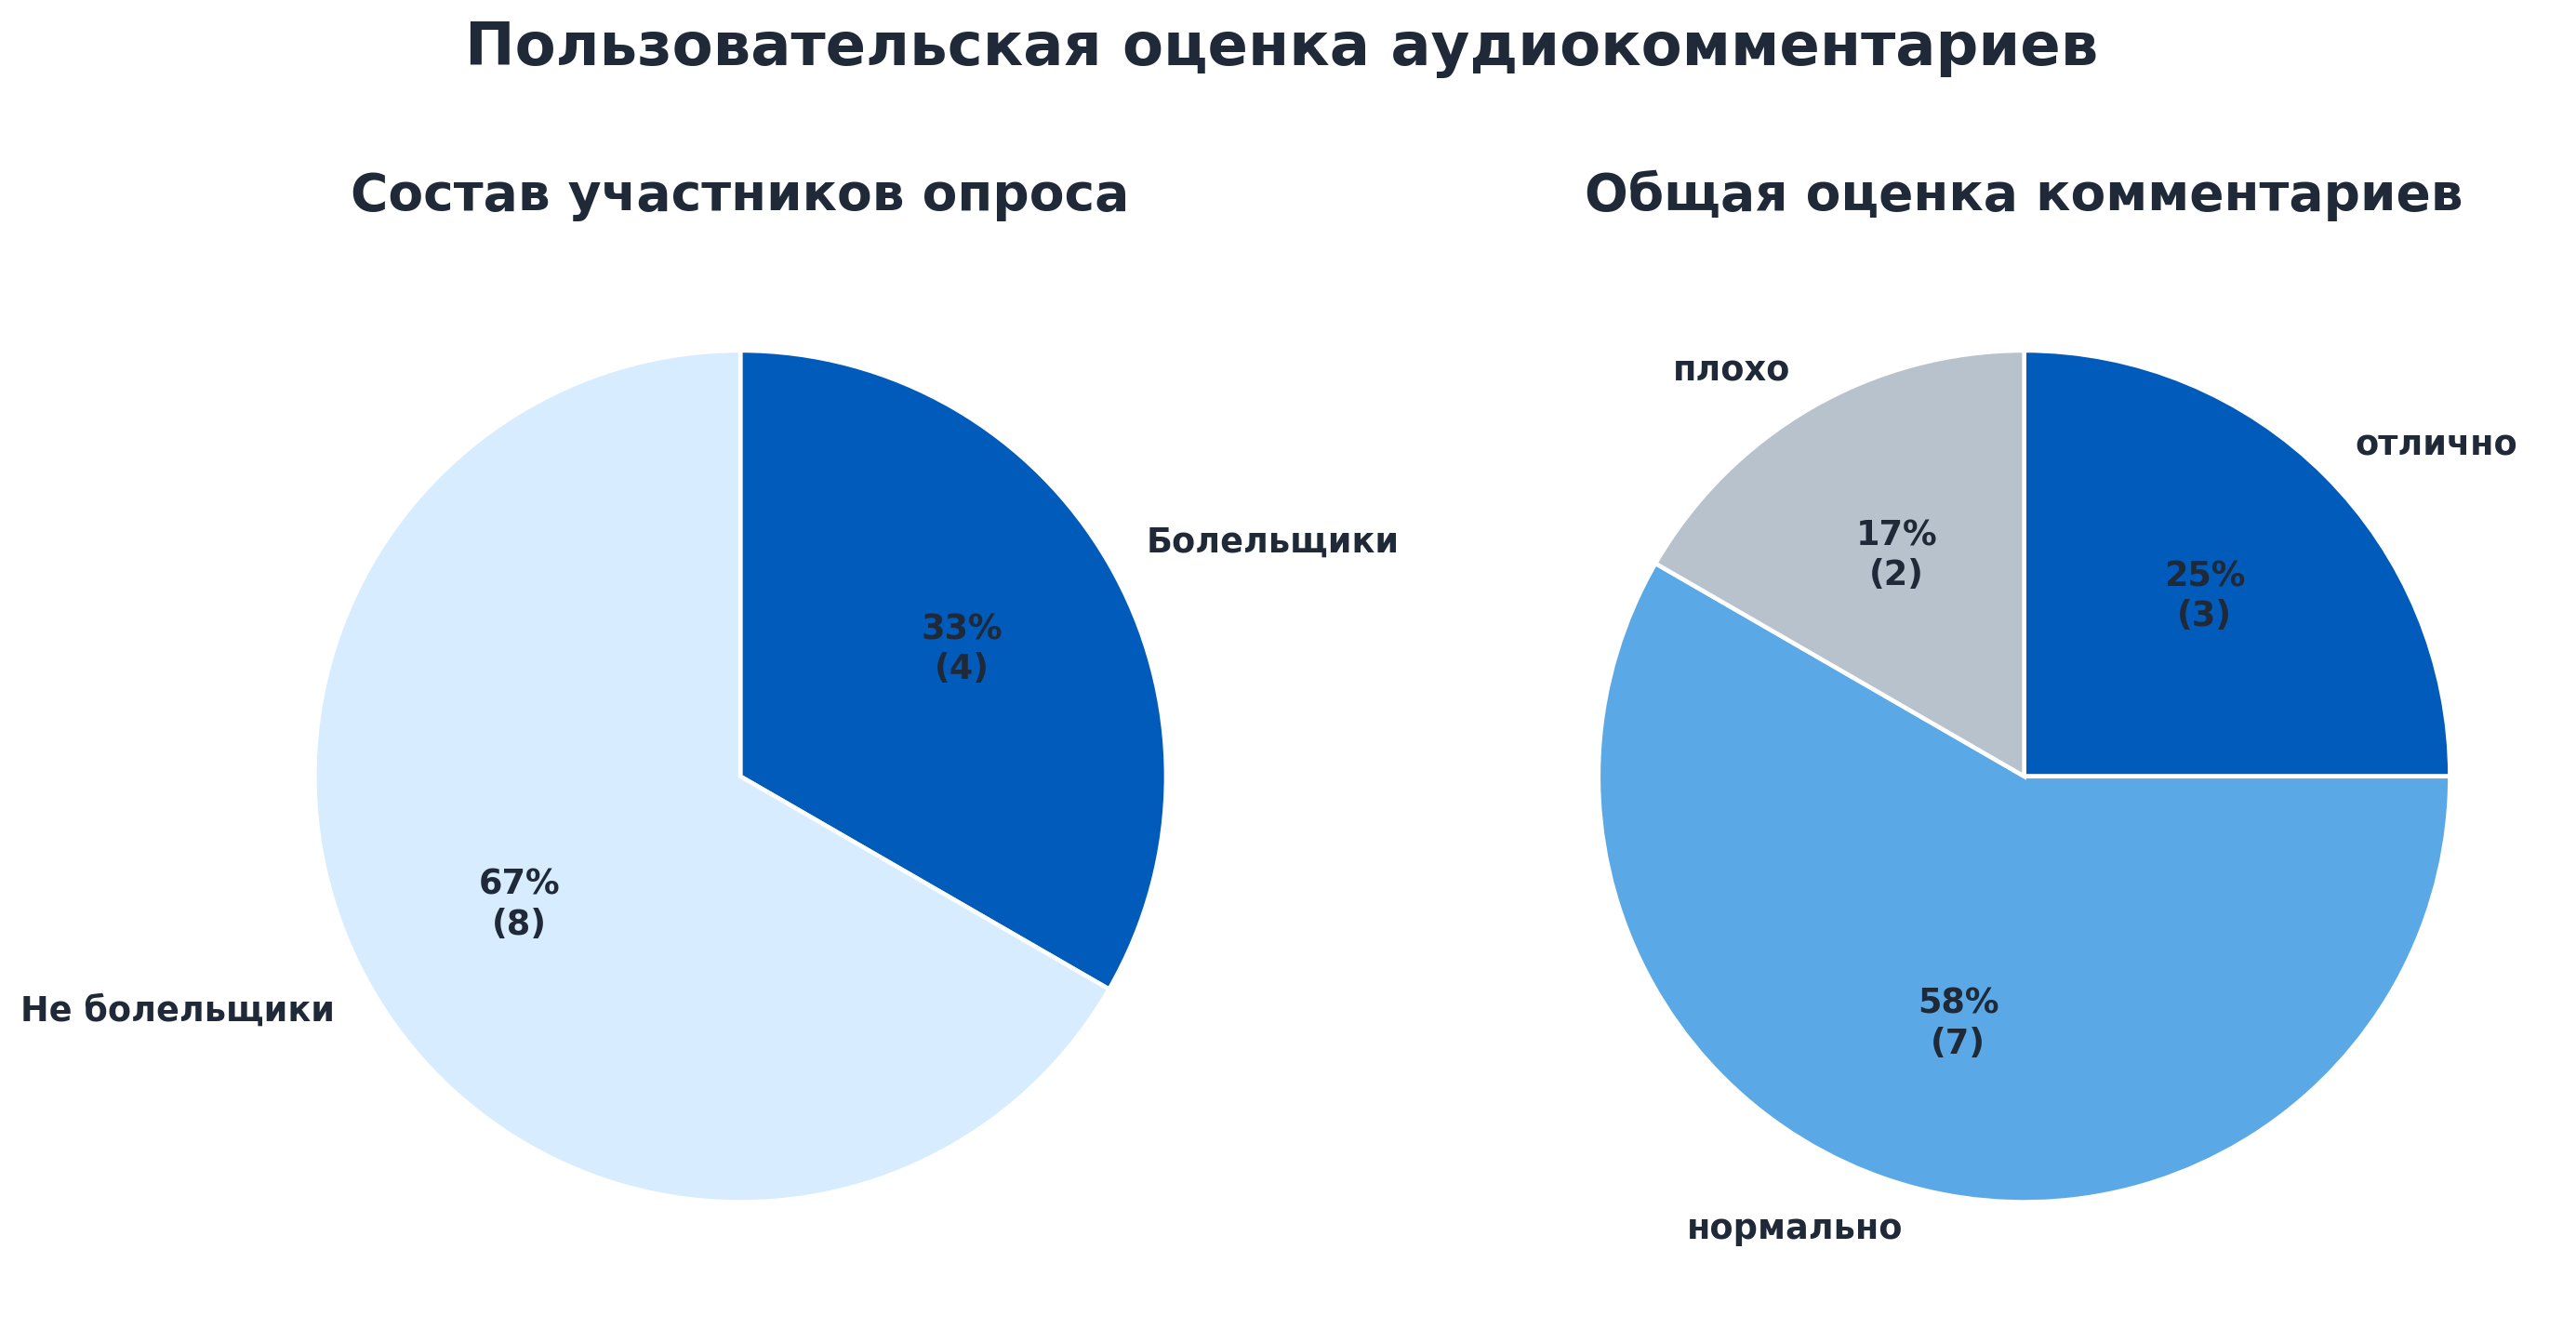
\includegraphics[width=0.82\textwidth]{survey_pie_charts.png}
\caption{Результаты пользовательской оценки аудиокомментариев}
\label{fig:survey}
\end{figure}

Мини-опрос используется как качественная проверка воспринимаемости результата. Участники оценивают комментарий по шкале «отлично» / «нормально» / «плохо» и оставляют свободный комментарий. Отдельно анализируются ответы футбольных болельщиков и участников без регулярного футбольного контекста.

% =========================
% ПРОТОТИП СИСТЕМЫ
% =========================
\section{Программный прототип}\label{sec:system}

\subsection{Структура проекта}

Прототип включает набор Jupyter-ноутбуков и вспомогательных модулей:

\begin{itemize}
    \item пайплайн загрузки и стандартизации матчей Евро-2024;
    \item модуль визуализации событий и StatsBomb~360;
    \item эксперименты по группировке цепочек и обучению селектора;
    \item ноутбук генерации LLM-комментариев через GigaChat API;
    \item ноутбук сборки аудиодорожки через Silero TTS;
    \item Streamlit-приложение для просмотра матчевых визуализаций.
\end{itemize}

\subsection{Интерфейс просмотра событий}

Streamlit-приложение позволяет выбрать матч, тайм и кадр, после чего отображает стандартизированную визуализацию события: положение актёра, игроков из 360-контекста, видимую область и направление действия. Это использовалось как инструмент валидации координат и отладки bad\_ids. На главной странице прототипа также размещаются видеофрагмент матча и готовая аудиодорожка тифлокомментария.

\begin{figure}[H]
\centering
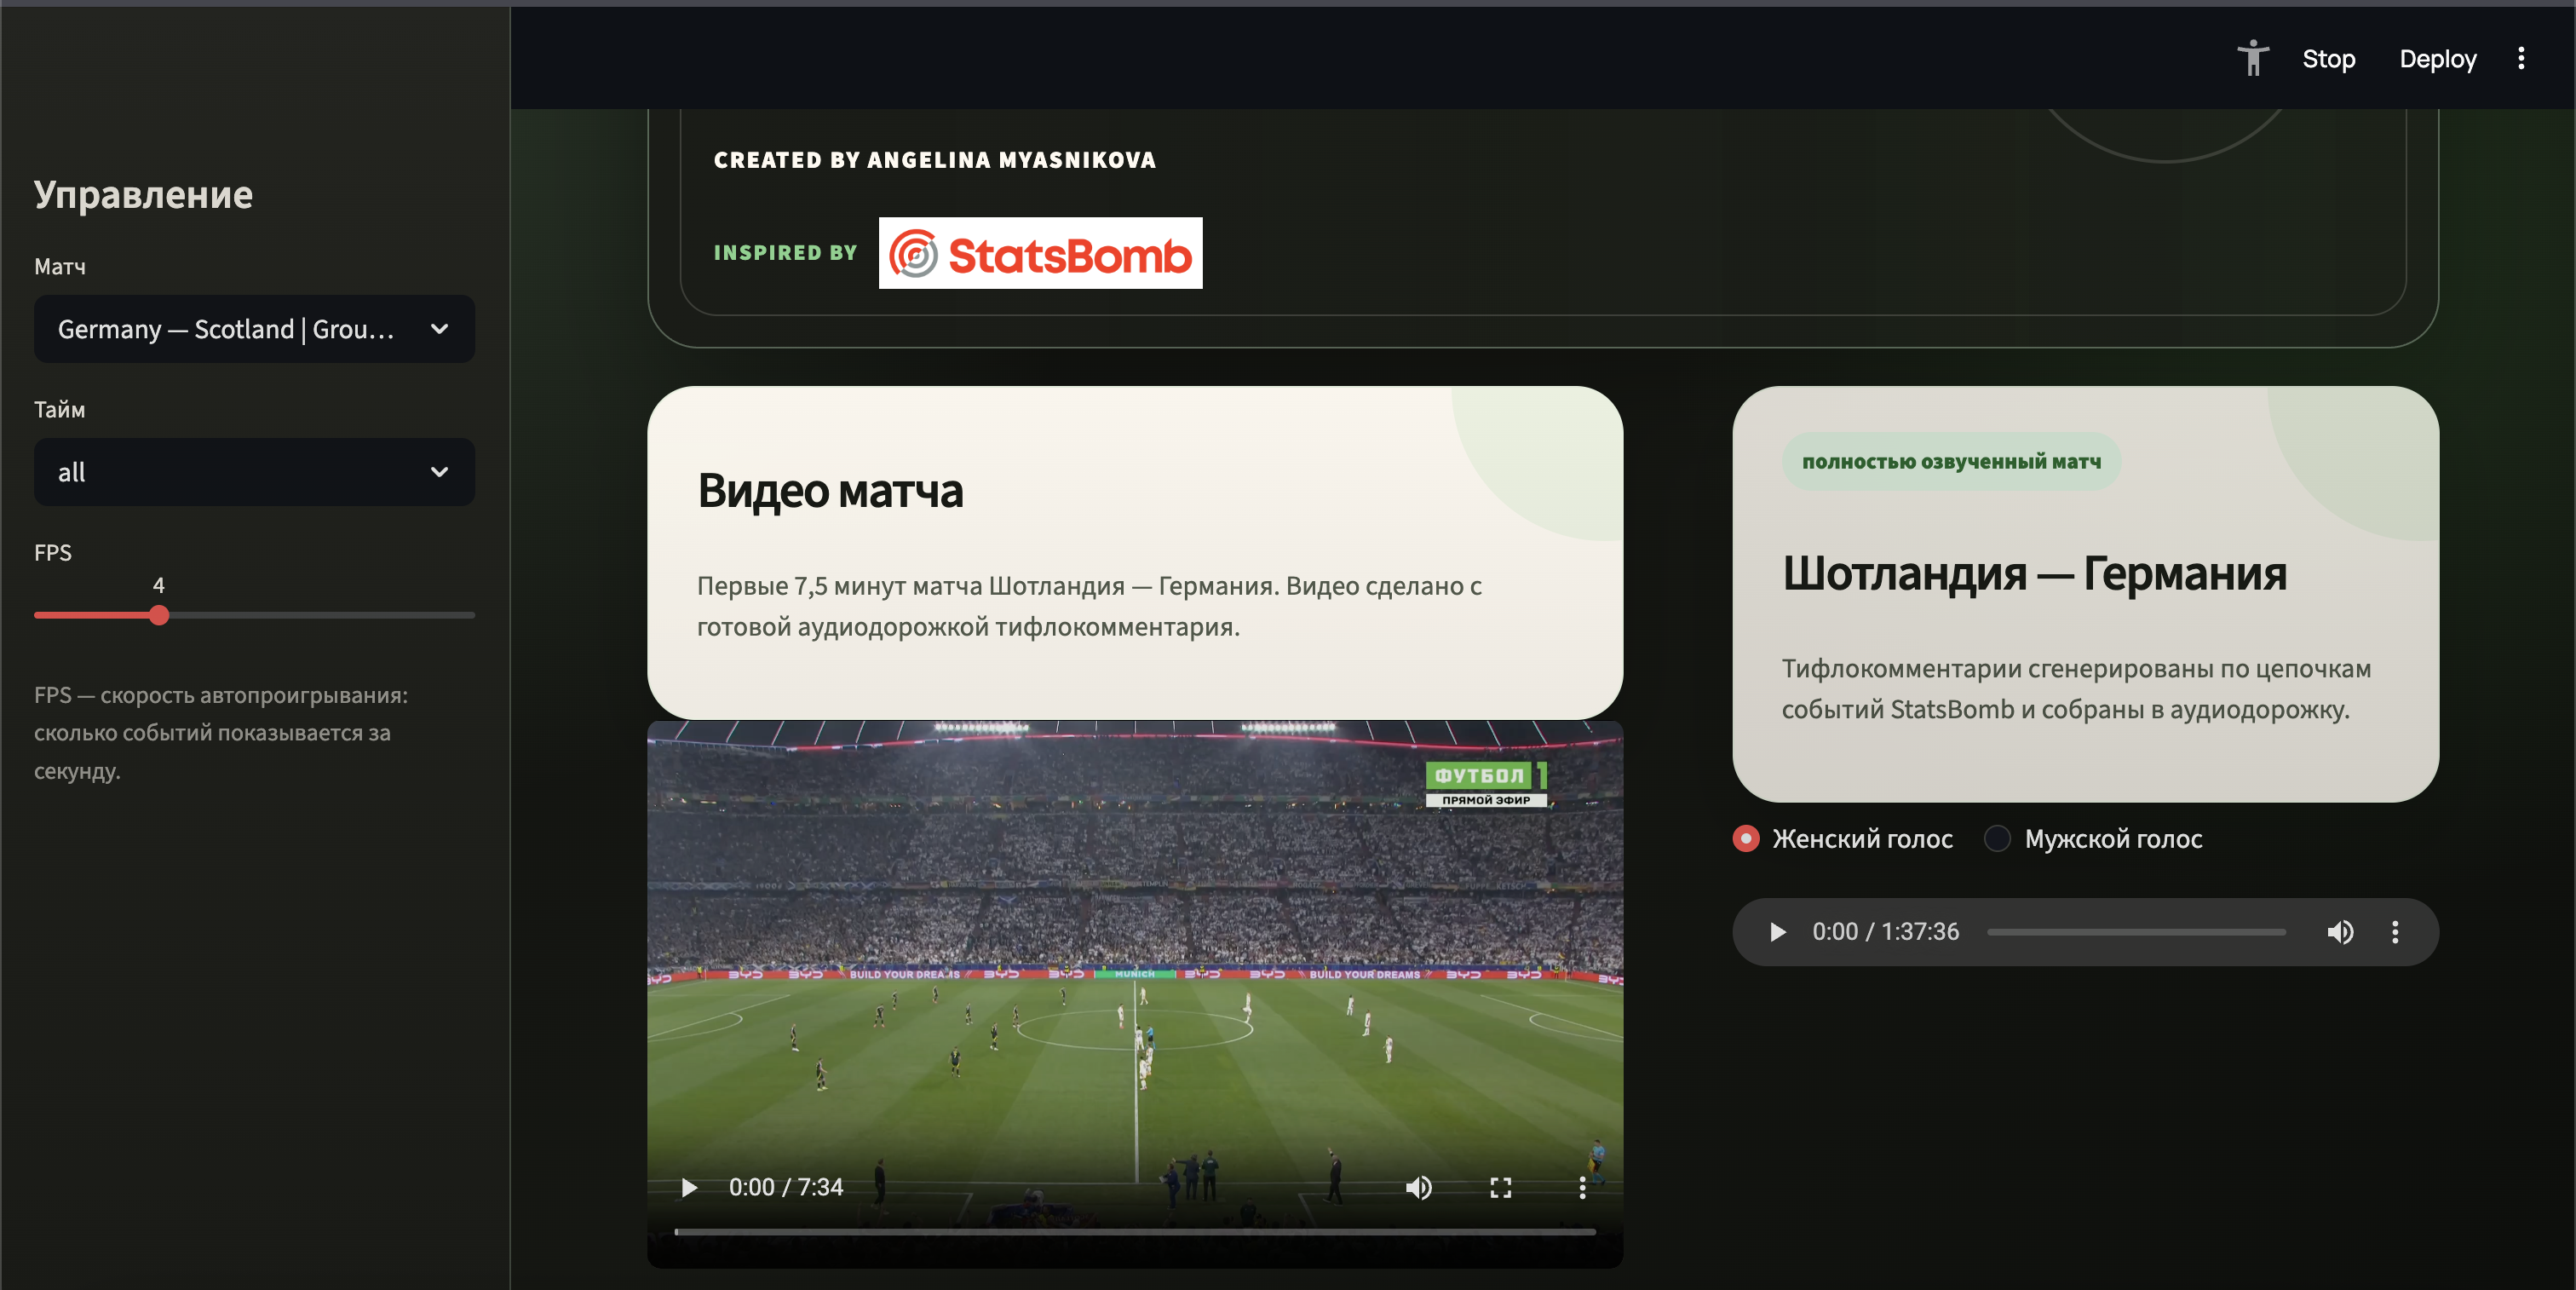
\includegraphics[width=0.92\textwidth]{demo1.png}
\caption{Главная страница Streamlit-приложения с видеофрагментом и аудиодорожкой}
\label{fig:streamlit-demo-main}
\end{figure}

\begin{figure}[H]
\centering
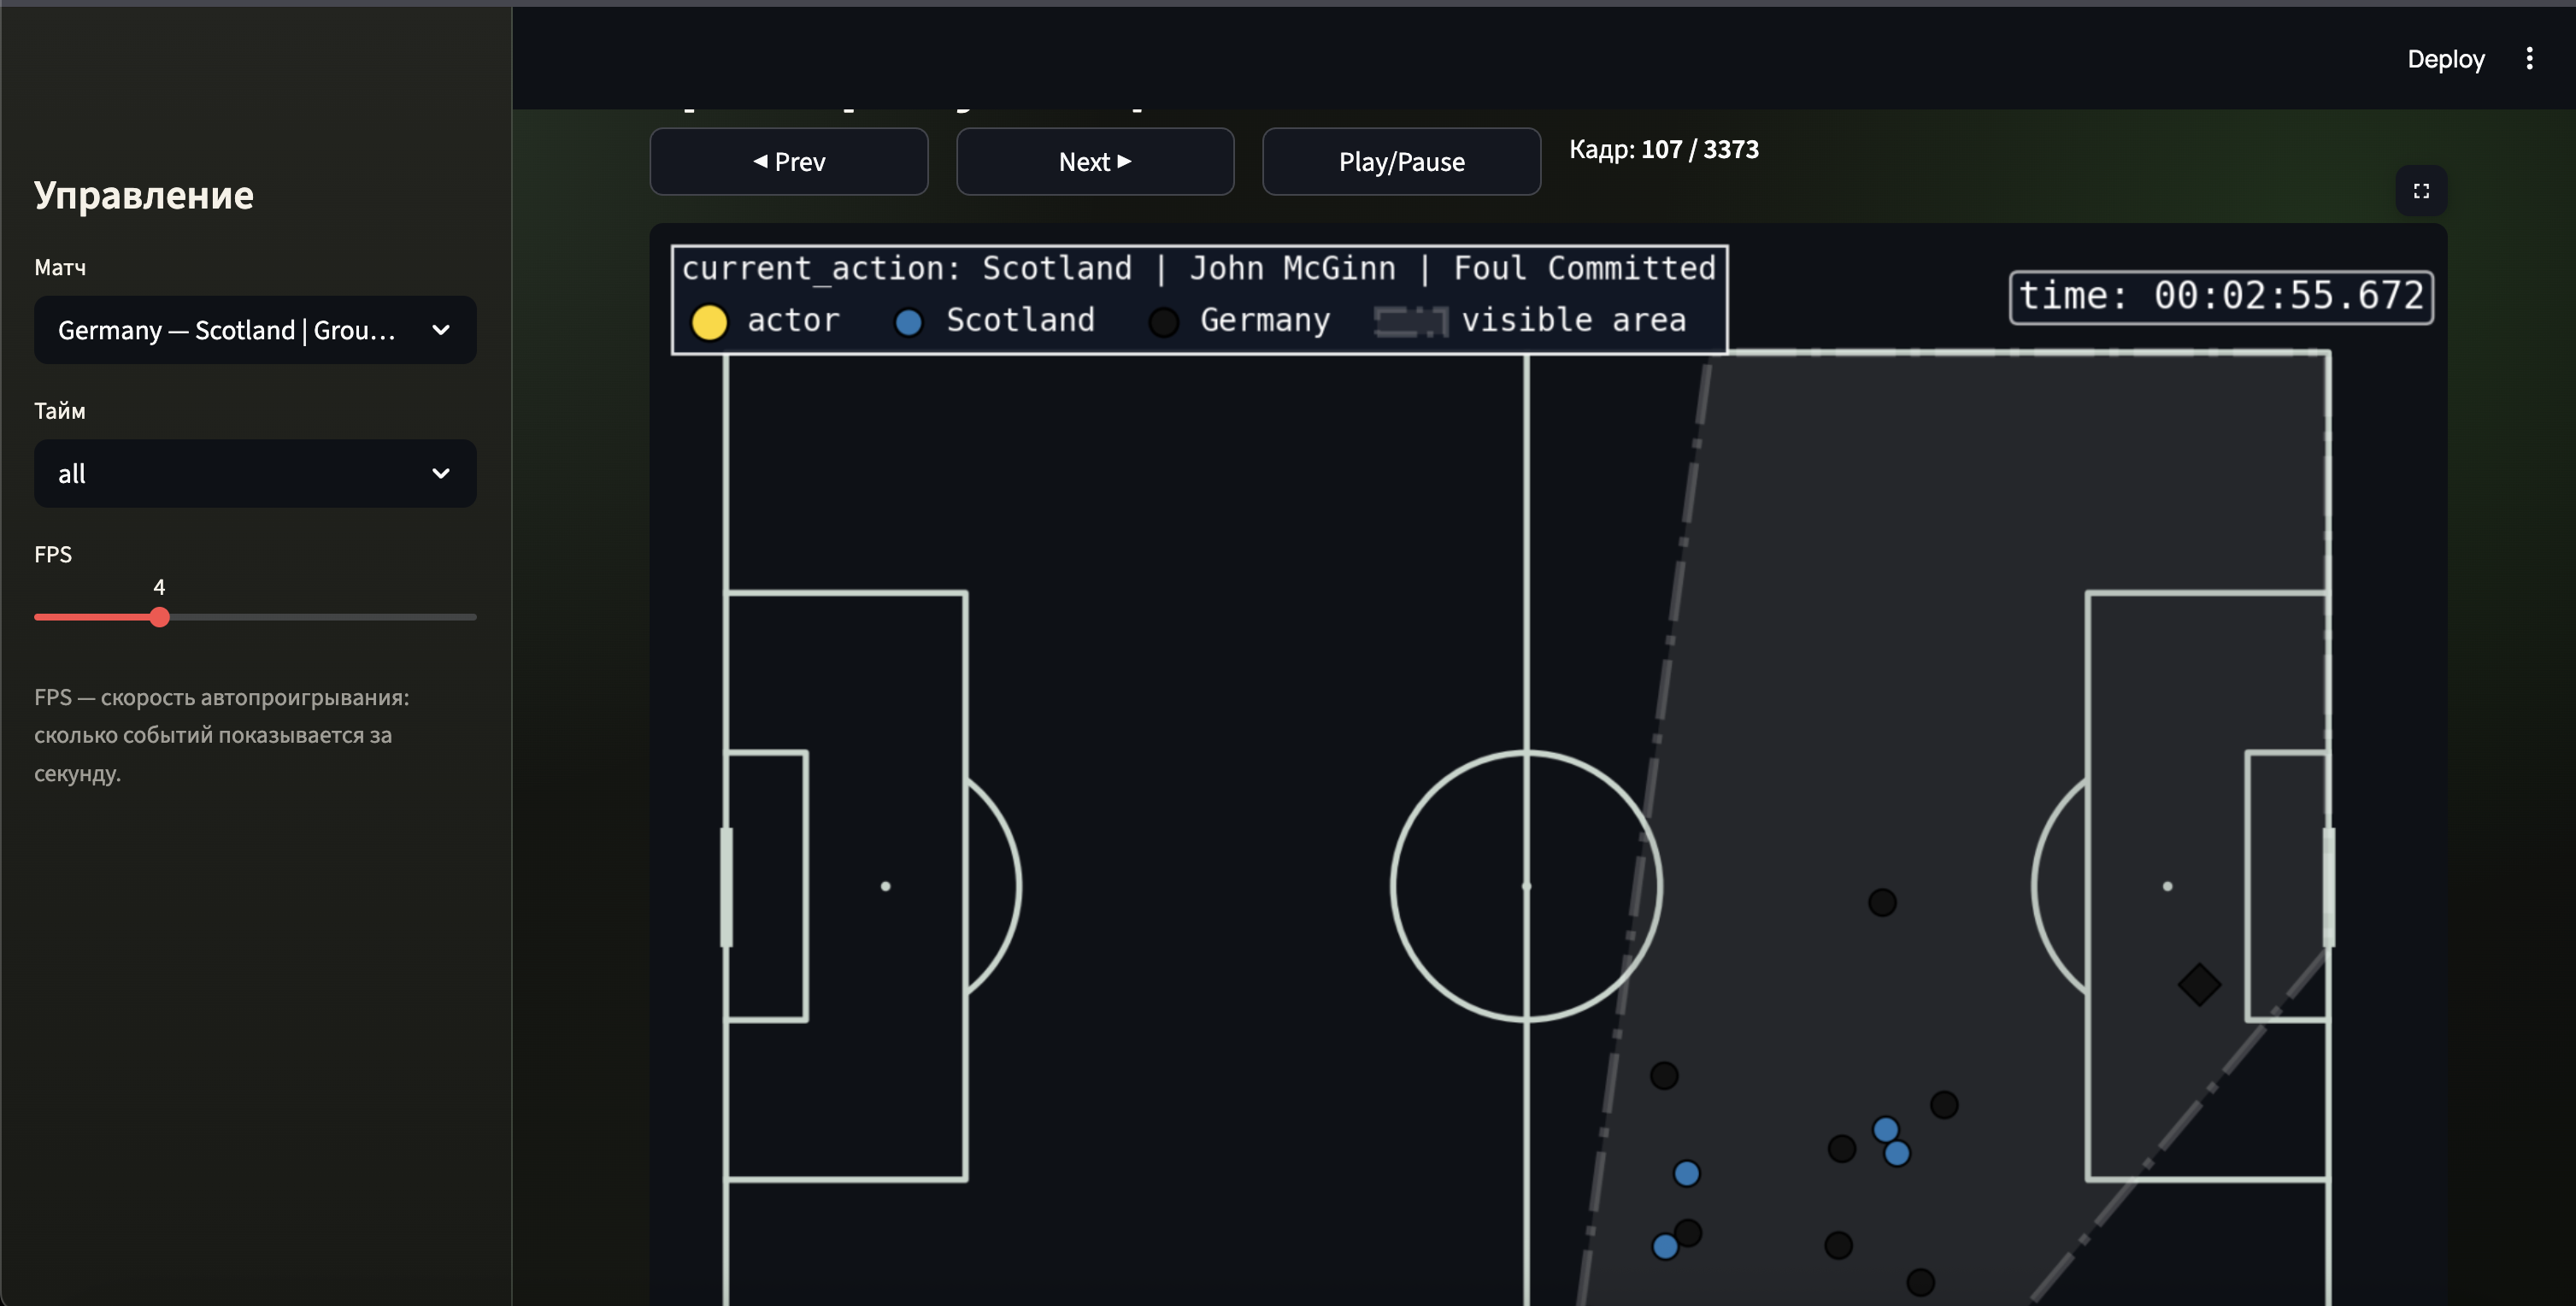
\includegraphics[width=0.92\textwidth]{demo2.png}
\caption{Страница просмотра визуализаций событий матча в Streamlit-приложении}
\label{fig:streamlit-demo-visualization}
\end{figure}

\subsection{Сборка аудиодорожки}

После генерации комментариев JSONL преобразуется в аудио. Для каждой реплики создаётся отдельный WAV-файл, затем комментарии размещаются на дорожке в соответствии с \texttt{t\_start}. В промежутках без комментариев добавляется тихий фоновый шум. Итогом являются отдельные дорожки по таймам и полный WAV-файл матча.

Для синтеза речи выбран Silero TTS: это открытая русскоязычная TTS-модель, которую можно запускать локально или в Kaggle без отдельного коммерческого сервиса. Для задачи футбольного аудиоописания важна также возможность управлять темпом речи: комментарии можно ускорять, чтобы реплика помещалась в короткое окно между игровыми событиями и не перекрывала следующий эпизод.

% =========================
% ЗАКЛЮЧЕНИЕ
% =========================
\section{Заключение}

В работе разработан прототип системы генерации русскоязычных тифлокомментариев по футбольным событиям StatsBomb. Реализованы стандартизация координат с учётом таймов, фильтрация некорректных 360-кадров, несколько стратегий группировки событий, эвристическая soft-разметка важности эпизодов, модели отбора, LLM-генерация комментариев и сборка аудиодорожки.

Эксперименты показали, что качество комментария существенно зависит от стратегии формирования эпизодов. Наиболее практичной оказалась стратегия \texttt{related\_stop\_cap}, совмещающая связность \texttt{related\_events} с ограничением длины и естественными стоп-событиями. Такой подход уменьшает риск длинных перегруженных payloads и делает вход для LLM более стабильным.

Ограничения работы связаны с отсутствием полноценной gold-разметки тифлокомментариев, использованием эвристических soft-labels и ограниченным пользовательским тестированием. В дальнейшем систему можно улучшить за счёт ручной разметки подвыборки эпизодов, LLM-as-a-judge оценки, расширения TTS-пайплайна и интеграции трекинговых данных при их наличии.

\newpage
\printbibliography[heading=bibintoc]

\newpage
\appendix
\renewcommand{\thesection}{\Alph{section}}
\renewcommand{\thetable}{\Alph{section}.\arabic{table}}
\renewcommand{\thefigure}{\Alph{section}.\arabic{figure}}

\section{Словарь признаков}\label{app:features}

В таблице ниже приведены признаки, сформированные после стандартизации событий и используемые для soft-разметки и обучения моделей отбора. Признаки с типом \texttt{target} не передаются в модель как входные переменные, а используются как целевые метки.

\begin{landscape}
\scriptsize
\setlength{\tabcolsep}{4pt}
\begin{longtable}{>{\raggedright\arraybackslash}p{0.15\linewidth}>{\raggedright\arraybackslash}p{0.24\linewidth}>{\raggedright\arraybackslash}p{0.13\linewidth}>{\raggedright\arraybackslash}p{0.40\linewidth}}
\caption{Итоговый словарь признаков эпизода}\label{tab:feature-dictionary}\\
\toprule
\textbf{Группа} & \textbf{Признак} & \textbf{Тип} & \textbf{Как рассчитывается и зачем нужен} \\
\midrule
\endfirsthead
\toprule
\textbf{Группа} & \textbf{Признак} & \textbf{Тип} & \textbf{Как рассчитывается и зачем нужен} \\
\midrule
\endhead
Структура эпизода & \texttt{duration\_sec} & числовой & Разность времени последнего и первого события. \\
Структура эпизода & \texttt{events\_n} & числовой & Количество событий внутри цепочки. \\
Структура эпизода & \texttt{first\_type} & категориальный & Тип первого события в цепочке. \\
Структура эпизода & \texttt{last\_type} & категориальный & Тип последнего события в цепочке. \\
Структура эпизода & \texttt{max\_gap\_sec} & числовой & Максимальный временной разрыв между соседними событиями. \\
Структура эпизода & \texttt{mean\_gap\_sec} & числовой & Средний временной разрыв между соседними событиями. \\
Структура эпизода & \texttt{period} & категориальный & Тайм первого события цепочки. \\
Структура эпизода & \texttt{stage} & категориальный & Стадия турнира из метаданных матча. \\
Типы событий & \texttt{class\_build\_up\_n} & числовой & Количество событий, отнесённых к семантическому классу build\_up. \\
Типы событий & \texttt{class\_defensive\_action\_n} & числовой & Количество событий, отнесённых к семантическому классу defensive\_action. \\
Типы событий & \texttt{class\_discipline\_n} & числовой & Количество событий, отнесённых к семантическому классу discipline. \\
Типы событий & \texttt{class\_duel\_n} & числовой & Количество событий, отнесённых к семантическому классу duel. \\
Типы событий & \texttt{class\_foul\_n} & числовой & Количество событий, отнесённых к семантическому классу foul. \\
Типы событий & \texttt{class\_low\_signal\_n} & числовой & Количество событий, отнесённых к семантическому классу low\_signal. \\
Типы событий & \texttt{class\_meta\_n} & числовой & Количество событий, отнесённых к семантическому классу meta. \\
Типы событий & \texttt{class\_set\_piece\_or\_ref\_n} & числовой & Количество событий, отнесённых к семантическому классу set\_piece\_or\_ref. \\
Типы событий & \texttt{class\_shot\_n} & числовой & Количество событий, отнесённых к семантическому классу shot. \\
Типы событий & \texttt{class\_transition\_n} & числовой & Количество событий, отнесённых к семантическому классу transition. \\
Типы событий & \texttt{class\_turnover\_n} & числовой & Количество событий, отнесённых к семантическому классу turnover. \\
Типы событий & \texttt{high\_event\_n} & числовой & Счётчик событий высокой значимости: удар, фол, офсайд, перехват, подбор, потеря и т.д. \\
Типы событий & \texttt{low\_signal\_n} & числовой & Счётчик низкосигнальных событий Ball Receipt* и Pressure. \\
Типы событий & \texttt{set\_play\_n} & числовой & Счётчик событий со стандартным play\_pattern: аут, штрафной, угловой, удар от ворот, kickoff. \\
Зоны поля & \texttt{center\_circle\_touch\_n} & числовой & Сколько событий произошло в центральном круге. \\
Зоны поля & \texttt{corner\_zone\_end\_n} & числовой & Сколько действий закончилось в угловой зоне. \\
Зоны поля & \texttt{ended\_final\_third\_n} & числовой & Сколько действий завершилось в финальной трети атаки. \\
Зоны поля & \texttt{entered\_opp\_box\_n} & числовой & Сколько раз действие вошло в чужую штрафную. \\
Зоны поля & \texttt{entered\_opp\_half\_n} & числовой & Сколько раз конечная зона события перешла на чужую половину. \\
Зоны поля & \texttt{left\_own\_box\_n} & числовой & Сколько раз действие вывело мяч из своей штрафной. \\
Зоны поля & \texttt{pre\_box\_end\_n} & числовой & Сколько действий закончилось перед штрафной. \\
Зоны поля & \texttt{third\_transition\_n} & числовой & Сколько действий перевело мяч между третями поля. \\
Зоны поля & \texttt{throwin\_end\_n} & числовой & Сколько действий закончилось у верхней или нижней бровки. \\
Движение мяча & \texttt{backward\_moves\_n} & числовой & Счётчик действий назад к своим воротам. \\
Движение мяча & \texttt{forward\_moves\_n} & числовой & Счётчик действий с положительным продвижением к чужим воротам. \\
Движение мяча & \texttt{lateral\_moves\_n} & числовой & Счётчик поперечных или фланговых перемещений. \\
Движение мяча & \texttt{long\_pass\_n} & числовой & Число передач, длина которых превышает порог длинной передачи. \\
Движение мяча & \texttt{max\_forward\_delta} & числовой & Максимальное продвижение к чужим воротам в одном действии цепочки. \\
Движение мяча & \texttt{mean\_abs\_lateral\_delta} & числовой & Среднее абсолютное поперечное смещение мяча. \\
Движение мяча & \texttt{mean\_forward\_delta} & числовой & Среднее продвижение к чужим воротам по событиям цепочки. \\
Движение мяча & \texttt{progressive\_carry\_n} & числовой & Число ведений мяча с заметным продвижением вперёд. \\
Движение мяча & \texttt{switched\_flank\_n} & числовой & Число действий, переведших мяч из одного флангового коридора в другой. \\
Исход действия & \texttt{bad\_pass\_outcome\_n} & числовой & Число передач с негативным outcome: Incomplete, Out, Pass Offside, Unknown. \\
Целевая метка & \texttt{soft\_label\_3} & target & Агрегация soft\_label\_5 в skip / brief / must. \\
Целевая метка & \texttt{soft\_label\_5} & target & Пятиуровневая эвристическая важность по формуле score. \\
\bottomrule
\end{longtable}
\end{landscape}


\section{Примеры JSON-payloads для LLM}\label{app:payloads}

В этом приложении приведены сокращённые примеры структур, которые используются в пайплайне. Полные JSON-файлы слишком объёмные для включения в текст работы, поэтому ниже оставлены только поля, важные для понимания методологии.

В этом приложении показан один и тот же эпизод на разных стадиях обработки. Пример взят из реального файла \texttt{llm\_payloads\_speak\_set\_related\_stop\_cap\_summary.json}: матч Германия --- Шотландия, стратегия \texttt{related\_stop\_cap}. В листингах не показаны все поля JSON, а оставлены только те, которые важны для понимания пайплайна.

\begin{lstlisting}[caption={Фрагмент исходного события StatsBomb до очистки},label={lst:raw-event-example}]
{
  "id": "df6f6fb7-f0b0-4561-9171-f4172f5e97e7",
  "index": 5,
  "period": 1,
  "timestamp": "00:00:01.191",
  "minute": 0,
  "second": 1,
  "type": {
    "id": 30,
    "name": "Pass"
  },
  "play_pattern": {
    "id": 9,
    "name": "From Kick Off"
  },
  "team": {
    "id": 770,
    "name": "Germany"
  },
  "player": {
    "id": 8966,
    "name": "Kai Havertz"
  },
  "position": {
    "id": 23,
    "name": "Center Forward"
  },
  "location": [
    61.0,
    40.1
  ],
  "duration": 1.234945,
  "related_events": [
    "f9195e75-1617-478c-bf9d-66f17151724a"
  ],
  "pass": {
    "recipient": {
      "id": 12407,
      "name": "Maximilian Mittelst\u00e4dt"
    },
    "length": 18.603764,
    "angle": -2.4475427,
    "height": {
      "id": 1,
      "name": "Ground Pass"
    },
    "end_location": [
      46.7,
      28.2
    ],
    "body_part": {
      "id": 38,
      "name": "Left Foot"
    },
    "type": {
      "id": 65,
      "name": "Kick Off"
    }
  }
}
\end{lstlisting}

\begin{lstlisting}[caption={То же событие после стандартизации и очистки полей},label={lst:clean-event-example}]
{
  "id": "df6f6fb7-f0b0-4561-9171-f4172f5e97e7",
  "index": 5,
  "period": 1,
  "timestamp": "00:00:01.191",
  "minute": 0,
  "second": 1,
  "type": {
    "name": "Pass"
  },
  "play_pattern": {
    "name": "From Kick Off"
  },
  "team": {
    "name": "Germany"
  },
  "player": {
    "id": 8966,
    "name": "Havertz",
    "jersey_number": 7
  },
  "position": {
    "name": "Center Forward"
  },
  "location": [
    59.0,
    39.9
  ],
  "duration": 1.234945,
  "related_events": [
    "f9195e75-1617-478c-bf9d-66f17151724a"
  ],
  "_flip180": true,
  "_reference_team": "Scotland",
  "pass": {
    "recipient": {
      "name": "Mittelst\u00e4dt"
    },
    "length": 18.603764,
    "height": {
      "name": "Ground Pass"
    },
    "end_location": [
      73.3,
      51.8
    ],
    "body_part": {
      "name": "Left Foot"
    },
    "type": {
      "name": "Kick Off"
    }
  }
}
\end{lstlisting}

\begin{lstlisting}[caption={Добавленные производные признаки для события},label={lst:derived-event-example}]
{
  "quality_flags": {
    "sb360_is_bad_filtered": 0,
    "skip_derive": 0,
    "skip_reason": null
  },
  "event_semantics": {
    "event_type": "Pass",
    "is_non_play": 0,
    "is_low_signal": 0,
    "is_key_action": 1
  },
  "orientation": {
    "period": 1,
    "team": "Germany",
    "own_goal_x": 120.0,
    "opp_goal_x": 0.0,
    "attack_sign": -1
  },
  "zones": {
    "start_abs": "center_circle_zone",
    "end_abs": "right_half:center_lane",
    "start_rel": "center_line",
    "end_rel": "own_half",
    "start_lane": "center_lane",
    "end_lane": "center_lane",
    "zone_transition": "center_line->own_half"
  },
  "movement": {
    "dx": 14.299999999999997,
    "dy": 11.899999999999999,
    "forward_delta": -14.299999999999997,
    "lateral_delta": 11.899999999999999,
    "label": "backward",
    "compass": "backward_left"
  },
  "episode_signals": {
    "is_long_pass": 0,
    "pass_length": 18.603764,
    "pass_style_ru": "\u043d\u0438\u0437\u043e\u043c",
    "pass_height_name": "Ground Pass",
    "pass_recipient": "Mittelst\u00e4dt",
    "pass_direction_compass": "backward_left",
    "pass_target_abs": "right_half:center_lane",
    "pass_target_rel": "own_half",
    "switched_flank": 0,
    "entered_opponent_half": 0,
    "entered_opponent_box": 0
  }
}
\end{lstlisting}

\begin{lstlisting}[caption={Фрагмент реального payload эпизода для LLM},label={lst:llm-payload-example}]
{
  "match_id": "3930158",
  "strategy": "related_stop_cap",
  "chain_event_ids": [
    "df6f6fb7-f0b0-4561-9171-f4172f5e97e7",
    "f9195e75-1617-478c-bf9d-66f17151724a",
    "65072c25-9c61-441e-a51c-52856c51ca94",
    "01be895c-5835-4a8d-b99f-2a642f5d26dc"
  ],
  "selection": {
    "soft_label_5": 4,
    "soft_label_3": 2,
    "commenting_mode": "must"
  },
  "chain_features": {
    "events_n": 4,
    "high_events_n": 0,
    "set_play_events_n": 4,
    "low_events_n": 1,
    "entered_opponent_box_n": 0,
    "importance_score_rule": 3
  },
  "events": [
    {
      "event_json": {
        "id": "df6f6fb7-f0b0-4561-9171-f4172f5e97e7",
        "index": 5,
        "period": 1,
        "timestamp": "00:00:01.191",
        "minute": 0,
        "second": 1,
        "type": {
          "name": "Pass"
        },
        "play_pattern": {
          "name": "From Kick Off"
        },
        "team": {
          "name": "Germany"
        },
        "player": {
          "id": 8966,
          "name": "Havertz",
          "jersey_number": 7
        },
        "position": {
          "name": "Center Forward"
        },
        "location": [
          59.0,
          39.9
        ],
        "duration": 1.234945,
        "related_events": [
          "f9195e75-1617-478c-bf9d-66f17151724a"
        ],
        "_flip180": true,
        "_reference_team": "Scotland",
        "pass": {
          "recipient": {
            "name": "Mittelst\u00e4dt"
          },
          "length": 18.603764,
          "height": {
            "name": "Ground Pass"
          },
          "end_location": [
            73.3,
            51.8
          ],
          "body_part": {
            "name": "Left Foot"
          },
          "type": {
            "name": "Kick Off"
          }
        }
      },
      "sb360_summary": {
        "freeze_frame_n": 20,
        "teammates_n": 10,
        "opponents_n": 10,
        "keepers_n": 0,
        "visible_area_points_n": 7
      },
      "derived": {
        "quality_flags": {
          "sb360_is_bad_filtered": 0,
          "skip_derive": 0,
          "skip_reason": null
        },
        "event_semantics": {
          "event_type": "Pass",
          "is_non_play": 0,
          "is_low_signal": 0,
          "is_key_action": 1
        },
        "orientation": {
          "period": 1,
          "team": "Germany",
          "own_goal_x": 120.0,
          "opp_goal_x": 0.0,
          "attack_sign": -1
        },
        "zones": {
          "start_abs": "center_circle_zone",
          "end_abs": "right_half:center_lane",
          "start_rel": "center_line",
          "end_rel": "own_half",
          "start_lane": "center_lane",
          "end_lane": "center_lane",
          "zone_transition": "center_line->own_half"
        },
        "movement": {
          "dx": 14.299999999999997,
          "dy": 11.899999999999999,
          "forward_delta": -14.299999999999997,
          "lateral_delta": 11.899999999999999,
          "label": "backward",
          "compass": "backward_left"
        },
        "episode_signals": {
          "is_long_pass": 0,
          "pass_length": 18.603764,
          "pass_style_ru": "\u043d\u0438\u0437\u043e\u043c",
          "pass_height_name": "Ground Pass",
          "pass_recipient": "Mittelst\u00e4dt",
          "pass_direction_compass": "backward_left",
          "pass_target_abs": "right_half:center_lane",
          "pass_target_rel": "own_half",
          "switched_flank": 0,
          "entered_opponent_half": 0,
          "entered_opponent_box": 0
        }
      }
    },
    {
      "event_json": {
        "id": "f9195e75-1617-478c-bf9d-66f17151724a",
        "index": 6,
        "period": 1,
        "timestamp": "00:00:02.426",
        "minute": 0,
        "second": 2,
        "type": {
          "name": "Ball Receipt*"
        },
        "play_pattern": {
          "name": "From Kick Off"
        },
        "team": {
          "name": "Germany"
        },
        "player": {
          "id": 12407,
          "name": "Mittelst\u00e4dt",
          "jersey_number": 18
        },
        "position": {
          "name": "Left Back"
        },
        "location": [
          73.3,
          51.8
        ],
        "related_events": [
          "df6f6fb7-f0b0-4561-9171-f4172f5e97e7"
        ],
        "_flip180": true,
        "_reference_team": "Scotland"
      },
      "sb360_summary": {
        "freeze_frame_n": 20,
        "teammates_n": 10,
        "opponents_n": 10,
        "keepers_n": 0,
        "visible_area_points_n": 6
      },
      "derived": {
        "quality_flags": {
          "sb360_is_bad_filtered": 0,
          "skip_derive": 0,
          "skip_reason": null
        },
        "event_semantics": {
          "event_type": "Ball Receipt*",
          "is_non_play": 0,
          "is_low_signal": 1,
          "is_key_action": 0
        },
        "orientation": {
          "period": 1,
          "team": "Germany",
          "own_goal_x": 120.0,
          "opp_goal_x": 0.0,
          "attack_sign": -1
        },
        "zones": {
          "start_abs": "right_half:center_lane",
          "end_abs": null,
          "start_rel": "own_half",
          "end_rel": null,
          "start_lane": "center_lane",
          "end_lane": null,
          "zone_transition": null
        },
        "movement": {
          "dx": null,
          "dy": null,
          "forward_delta": null,
          "lateral_delta": null,
          "label": "unknown",
          "compass": "unknown"
        },
        "episode_signals": {
          "is_long_pass": 0,
          "pass_length": null,
          "pass_style_ru": null,
          "pass_height_name": null,
          "pass_recipient": null,
          "pass_direction_compass": null,
          "pass_target_abs": null,
          "pass_target_rel": null,
          "switched_flank": 1,
          "entered_opponent_half": 0,
          "entered_opponent_box": 0
        }
      }
    }
  ]
}
\end{lstlisting}

Смысл преобразования следующий. Исходный StatsBomb JSON содержит подробное описание одного действия, но в нём много полей, которые не нужны для генерации комментария. После очистки остаются факты, которые можно безопасно передать модели: время, команда, игрок, тип действия, координаты и исход. Затем добавляется блок \texttt{derived}: он не берётся из StatsBomb напрямую, а рассчитывается в работе. Именно в нём появляются направление атаки, относительные зоны поля, движение вперёд или назад, признаки длинной передачи, перевода фланга и входа в опасную зону. Финальный payload объединяет несколько связанных событий в эпизод, добавляет агрегированные признаки цепочки и режим комментирования.


\section{Системный промпт для генерации комментариев}\label{app:system-prompt}

В этом приложении приведён системный промпт, который использовался для генерации русскоязычных тифлокомментариев по выбранным payloads.

\begin{longtable}{p{0.24\textwidth}p{0.66\textwidth}}
\caption{Структура системного промпта для LLM-комментатора}
\label{tab:system-prompt-structure}\\
\toprule
\textbf{Блок промпта} & \textbf{Содержание инструкции} \\
\midrule
\endfirsthead

\toprule
\textbf{Блок промпта} & \textbf{Содержание инструкции} \\
\midrule
\endhead

\bottomrule
\endfoot

Роль модели & Модель задаётся как тифлокомментатор футбольного матча для незрячего слушателя. Ответ должен быть только на русском языке. \\
Входной JSON & Объясняется, что на вход передаётся не весь матч, а один выбранный payload: \texttt{match\_id}, \texttt{strategy}, \texttt{chain\_event\_ids}, \texttt{chain\_features}, \texttt{selection}, список \texttt{events}. \\
Решение отбора & Поле \texttt{selection.soft\_label\_3} интерпретируется как режим комментария: \texttt{brief} --- коротко прокомментировать, \texttt{must} --- обязательно отразить главное действие. Модель не должна объяснять soft-label или score в ответе. \\
Поля события & Модели перечисляются ключевые поля \texttt{event\_json}: время, тайм, тип события, команда, игрок, координаты, данные паса, ведения, удара, действия вратаря и стандарта. \\
Производные признаки & Объясняются \texttt{derived.orientation}, \texttt{derived.movement}, \texttt{derived.zones}, \texttt{derived.episode\_signals}. Отдельно указано, что движение «вперёд» и «назад» определяется относительно команды с мячом. \\
Стиль & Только настоящее время, нейтральный стиль, без местоимений «мы», «они», без эмоций и оценочных слов. Для \texttt{brief} --- одно короткое предложение, для \texttt{must} --- одно или максимум два предложения. \\
Запрещённые связки & Запрещены слова «затем», «потом», «после этого», «далее», «в итоге», «следом», «сначала», чтобы ответ звучал как live-комментарий, а не пересказ цепочки. \\
Приоритет действий & В первую очередь описываются удары, голы, сейвы, блоки, перехваты, потери, фолы, офсайды, стандарты и явное продвижение атаки. Низкосигнальные события \texttt{Ball Receipt*} и \texttt{Pressure} не должны становиться главным содержанием сами по себе. \\
Правила по типам & Отдельно заданы правила для \texttt{Pass}, \texttt{Carry}, \texttt{Shot}, \texttt{Goal Keeper}, \texttt{Block}, оборонительных действий, фолов, офсайдов и стандартов. Для паса требуется учитывать получателя, высоту, направление, целевую зону и негативный исход. \\
StatsBomb 360 & 360-контекст трактуется как моментный freeze-frame, а не видео. Его можно использовать только для простых фактов вроде давления или плотности игроков; имена и номера игроков из 360 придумывать нельзя. \\
Формат ответа & Требуется строго валидный JSON с полями \texttt{t\_start}, \texttt{t\_end}, \texttt{commentary}, \texttt{commented\_event\_ids}, \texttt{commented\_event\_types}. \\
\end{longtable}

Ниже приведена краткая версия ключевой инструкции, использованной в системном промпте:

\begin{quote}\small
Ты --- тифлокомментатор футбольного матча для незрячего слушателя. Тебе передаётся один JSON payload футбольного эпизода. Эпизод уже выбран системой отбора; твоя задача --- не решать, нужно ли его комментировать, а кратко и фактически правильно озвучить выбранный эпизод. Отвечай только на русском языке, в настоящем времени, нейтрально, без слов «затем», «потом», «после этого». Используй только факты из \texttt{event\_json} и готовые интерпретации из \texttt{derived}. Если payload попал к тебе, его нужно прокомментировать. Верни строго валидный JSON без текста вне JSON.
\end{quote}


\section{Пример ответа LLM}\label{app:model-output}

Ниже приведён пример ответа модели GigaChat-2-Pro для одного payload матча Германия --- Шотландия. В основной пайплайн дальше передаются поля времени и текст комментария.

\begin{table}[H]
\centering
\small
\caption{Пример JSON-ответа модели после генерации комментария}
\label{tab:model-output-example}
\begin{tabular}{p{0.23\textwidth}p{0.67\textwidth}}
\toprule
Поле & Значение \\
\midrule
\texttt{t\_start} & \texttt{00:00:07.397} \\
\texttt{t\_end} & \texttt{00:00:07.871} \\
\texttt{commentary} & Хавертц делает пас низом после начального удара, но МакГрегор не может восстановить владение. \\
\bottomrule
\end{tabular}
\end{table}

В полном JSONL-файле этот ответ хранится вместе с технической информацией о стратегии группировки, номере payload, модели и статусе парсинга. Для сборки аудиодорожки используются прежде всего три поля: начало реплики, конец связанного эпизода и сам текст комментария.


\section{Материалы ручного анализа тифлокомментариев}\label{app:okko-analysis}

При формировании правил комментирования дополнительно просматривались спортивные трансляции с тифлокомментариями. Ниже приведён пример экрана Okko, использованный как ориентир для анализа пользовательского сценария.

\IfFileExists{graphics/okko.png}{%
\begin{figure}[H]
\centering
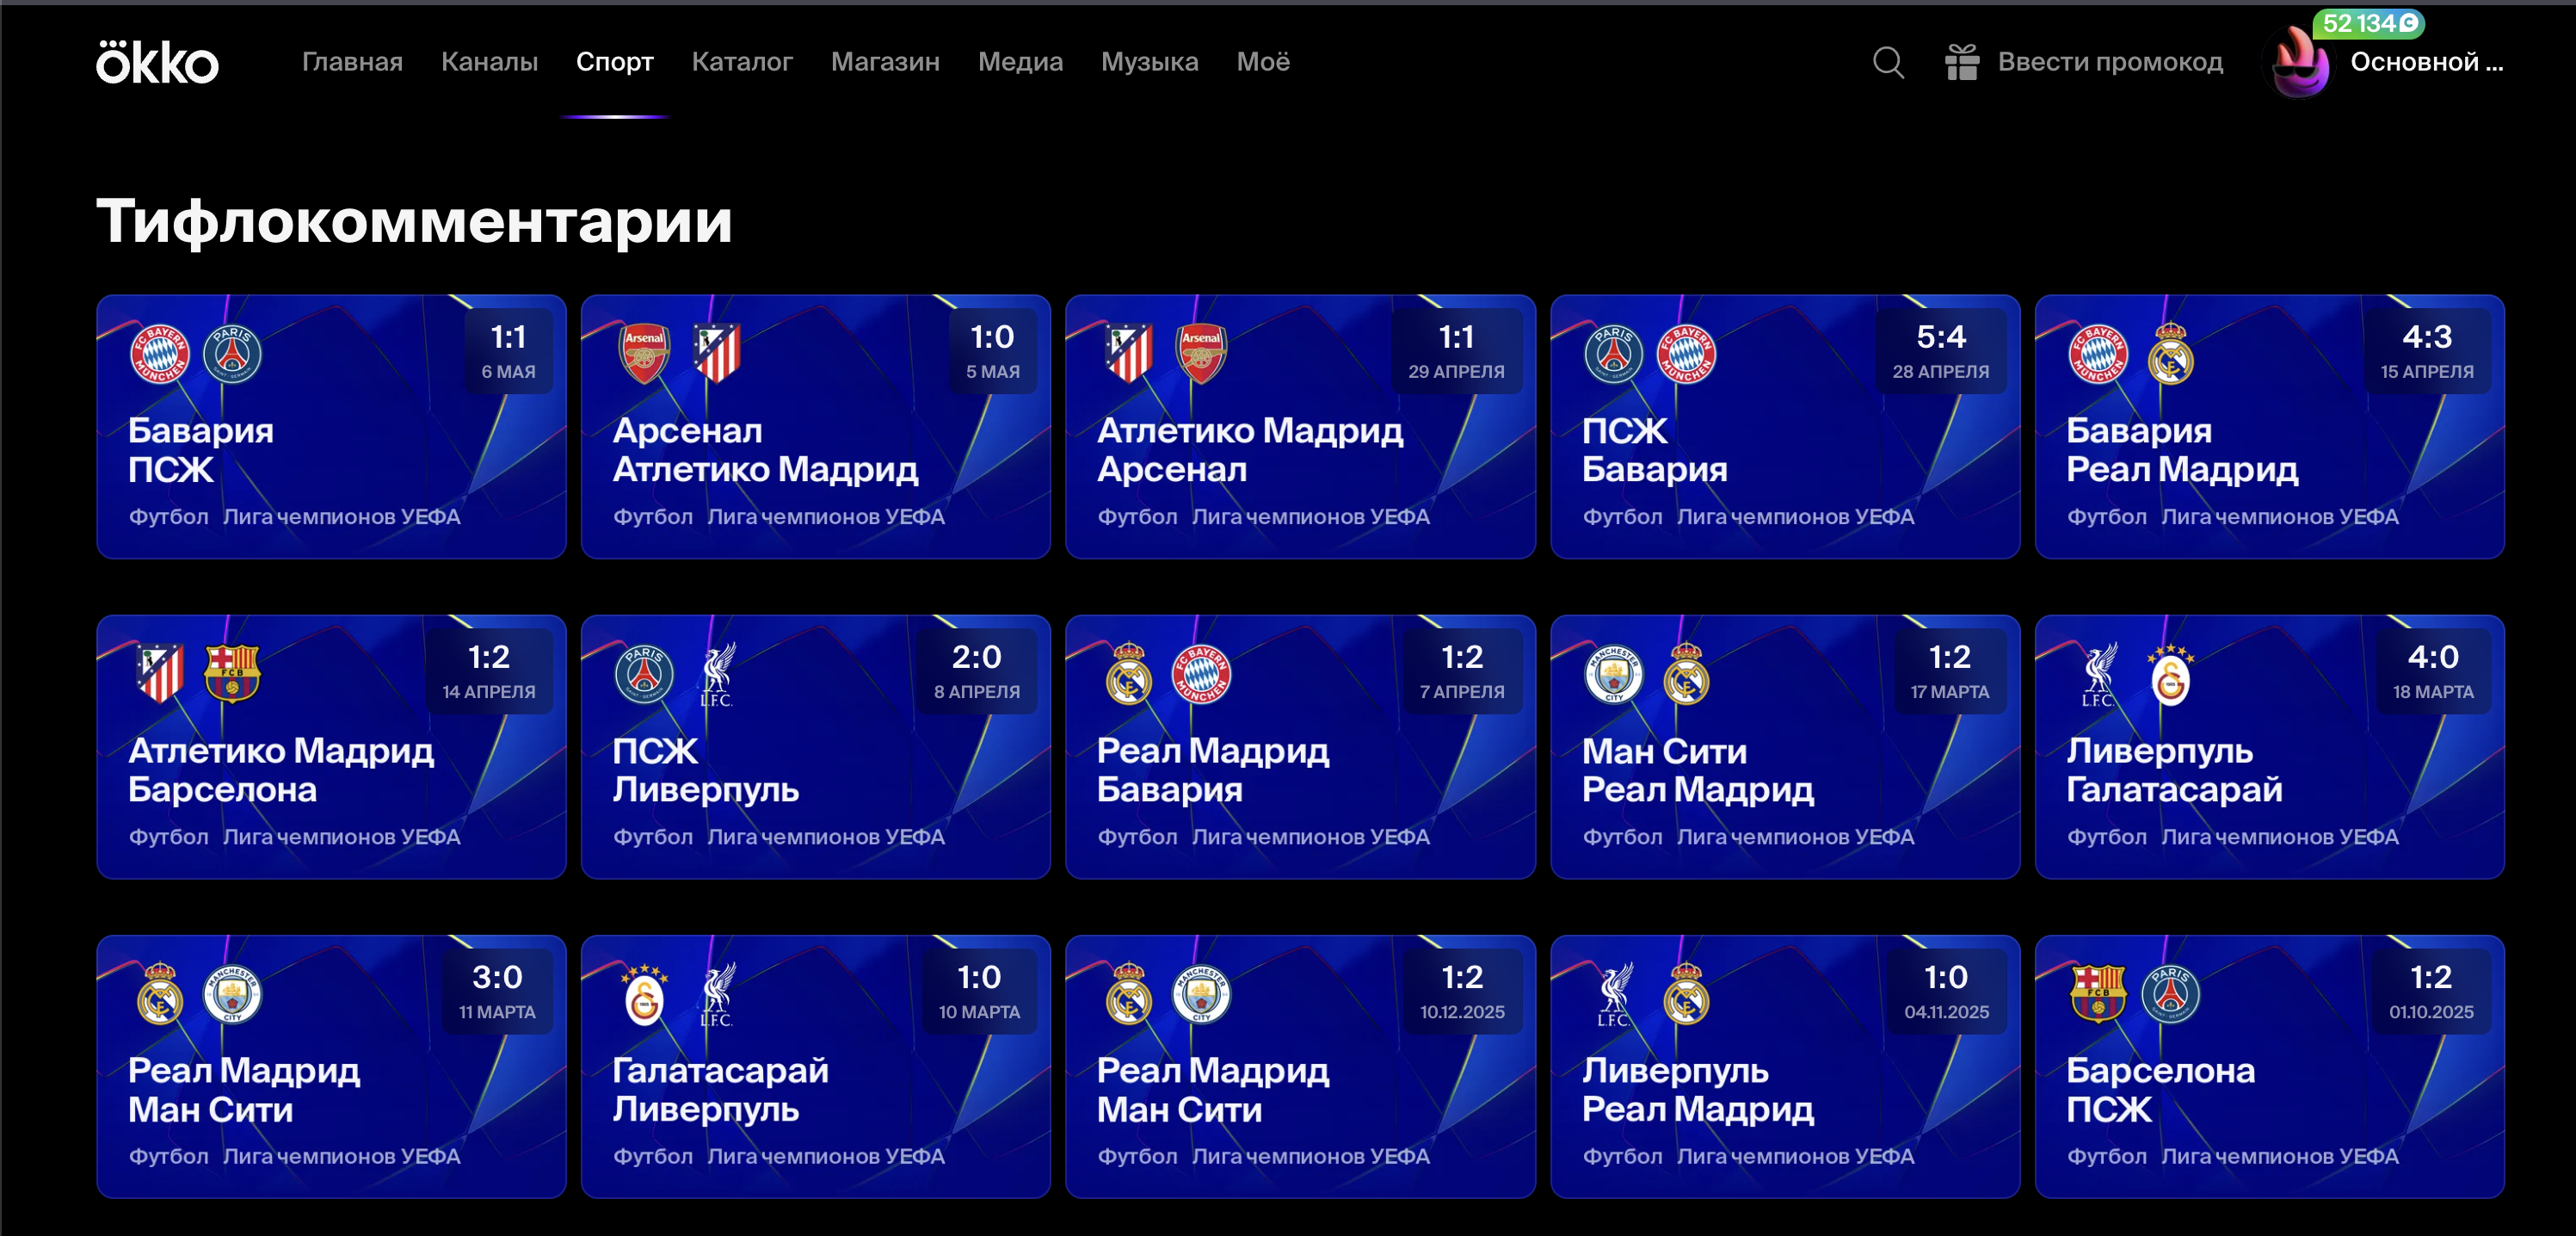
\includegraphics[width=0.92\textwidth]{okko.png}
\caption{Пример спортивной трансляции с тифлокомментарием в Okko}
\label{fig:okko-screenshot}
\end{figure}
}{%
\begin{center}
\fbox{\parbox{0.82\textwidth}{\centering Скриншот Okko не найден в папке \texttt{vkr/graphics}. Для вставки положите файл как \texttt{okko.png}.}}
\end{center}
}

\end{document}
